



\section{BL test case I}

In this section test case 1 is solved (1D incompressible 
BL equations with gas injection along a bore hole). 
The gas is injected at a velocity of $u_g \phi =1$ and 
a saturation of one $S_g=1$. On the outlet boundary the 
pressure level is set to zero. All boundary conditions are 
applied naturally. 

A converged time step of $1\times 10^{-3}$ is used for all simulations 
and applications with the continuous and discontinuous between 
element formulations are presented. All simulations 
use the overlapping mixed finite element method with a 
piecewise linear variation of the velocity within each 
element and quadatric pressure. Saturation is collocated at 
the pressure nodes. Although saturation is cacluated using 
a control volume formulation a FEM interpolation is 
used to form the high order fluxes and these are also 
used in this section for most of the graphs. 


\subsubsection{Continuous formulation}

{\it Upwind solution} 

In figure \ref{bl-exact-meth-upwind}  the 
control volume (CV) saturation of gas (with horizontal and vertical lines) and 
the quadratic finite element interpolation of these are 
presented. 
As can be seen the solution converges with increased resolution. 
Notice that the corners of the control volumes pass 
very closely 
to the converged solution. This is because upwinding of 
the velocities is used (or equivalently the relative permeabilities) 
and it is at these corners that the equations reach the 
balance necessary to match closely the analytical solution. 

{\it Optimal upwinding} 

If one uses 80$\%$ upwinding and 20$\%$ downwinding then 
one gets a closer match with the converged solution, 
see figure \ref{bl-exact-meth-cv-0-8-ele50} where we see the 
control volume solution and figure \ref{bl-optimal-upwind} 
and where these solutions with upwinding as well as 
the optimal quantity of upwinding (as described in section \ref{opt-up}) 
are compared. 
One should note that 80$\%$ upwinding matches quite closely with the 
optimal upwind parameter results and these results converge rapidly 
with increase resolution. When applying optimal upwinding 
the quantity of upwinding (upwind fraction) varies from 
1 (full upwinding) which is typically applied near shocks 
and $\frac{1}{2}$ which is central differencing. See 
the upwind fractions in figure \ref{bl-upwind-frac} for the 
different grid resolutions and each of the two phases. 
The upwind fraction is chosen so as to increase the accuracy 
of the formulation. However, even though downwinding of the 
velocity may increase this accuracy we limit ourselves to 
central difference. If however, one chooses to use 
upwinding and downwinding then one obtains the solution 
shown in figure \ref{bl-upwind-v-up-and-down}. Including 
the downwind components may not be consistent with the characteristics 
of the differential equation and thus may detract from 
its accurate solution. The optimal solution for a number 
of different resolutions ranging from 3 elements to 50 elements 
is shown in figure \ref{bl-3-10-20-50}. Notice that 
the solution converges rapidly. There are no oscillations in 
the corresponding control volume solutions, but here we are 
looking at the finite element interpolation (using a Galerkin 
project) of the control volume solution which does oscillate 
near the shock. 

 


% cty:


%fig1: bl-exact-meth-upwind.xmgr

%fig2: bl-exact-meth-cv-0-8-ele50.xmgr

%fig3: bl-optimal-upwind.xmgr

%fig4: bl-upwind-frac.xmgr

%fig5: bl-upwind-v-up-and-down.xmgr

%fig6: bl-3-10-20-50.xmgr


\begin{figure}[H]
\vbox{
\begin{center}
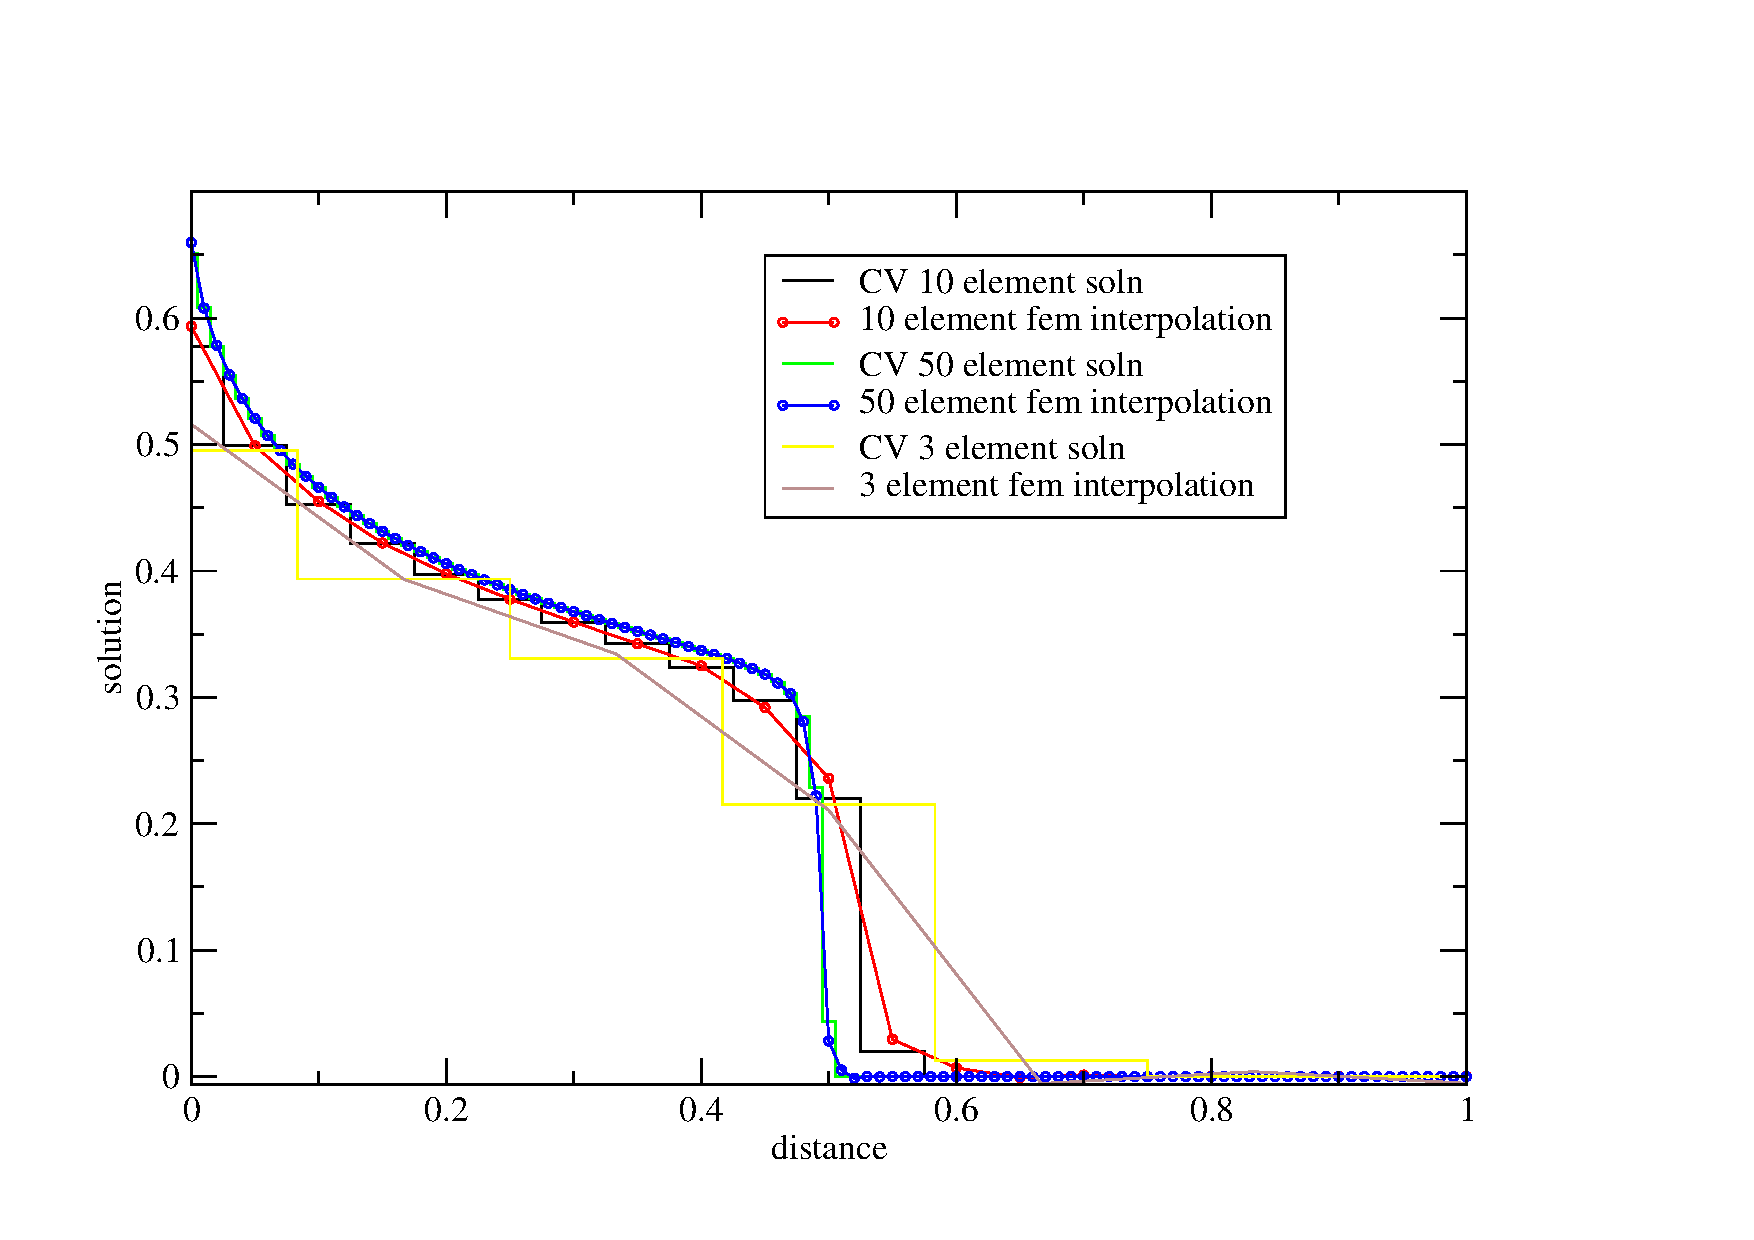
\includegraphics[width=17.5cm,height=12.5cm]{./doc_figures/bl-exact-meth-upwind}
\end{center}
\vspace{0.cm}}
\caption{The continuous upwind method applied to the BL test 
case 1 for different mesh resolutions.}
\label{bl-exact-meth-upwind}
\end{figure}

\begin{figure}[H]
\vbox{
\begin{center}
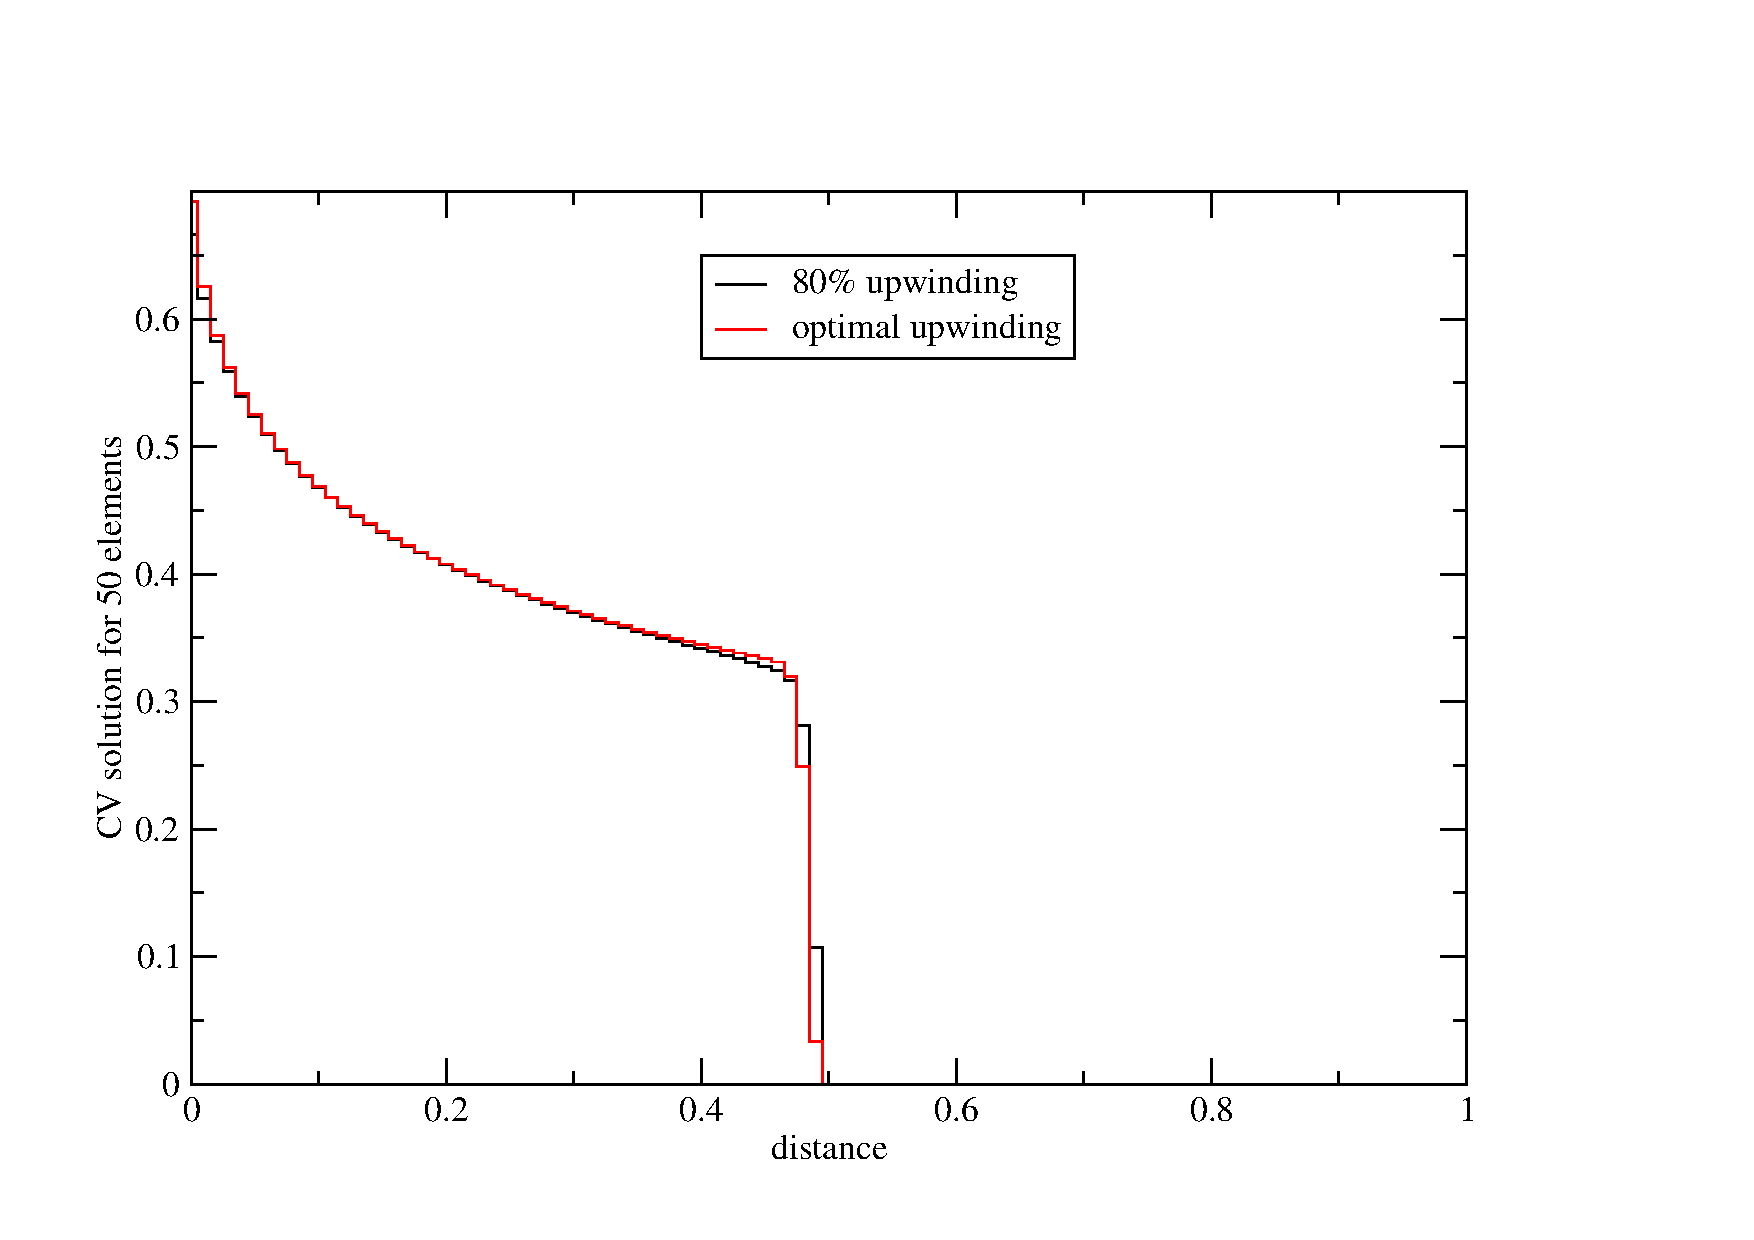
\includegraphics[width=17.5cm,height=12.5cm]{./doc_figures/bl-exact-meth-cv-0-8-ele50}
\end{center}
\vspace{0.cm}}
\caption{Comparison of the control volume solutions using 80$\%$ upwinding 
and with optimal upwinding and using 50 continuous quadatric elements. }
\label{bl-exact-meth-cv-0-8-ele50}
\end{figure}

\begin{figure}[H]
\vbox{
\begin{center}
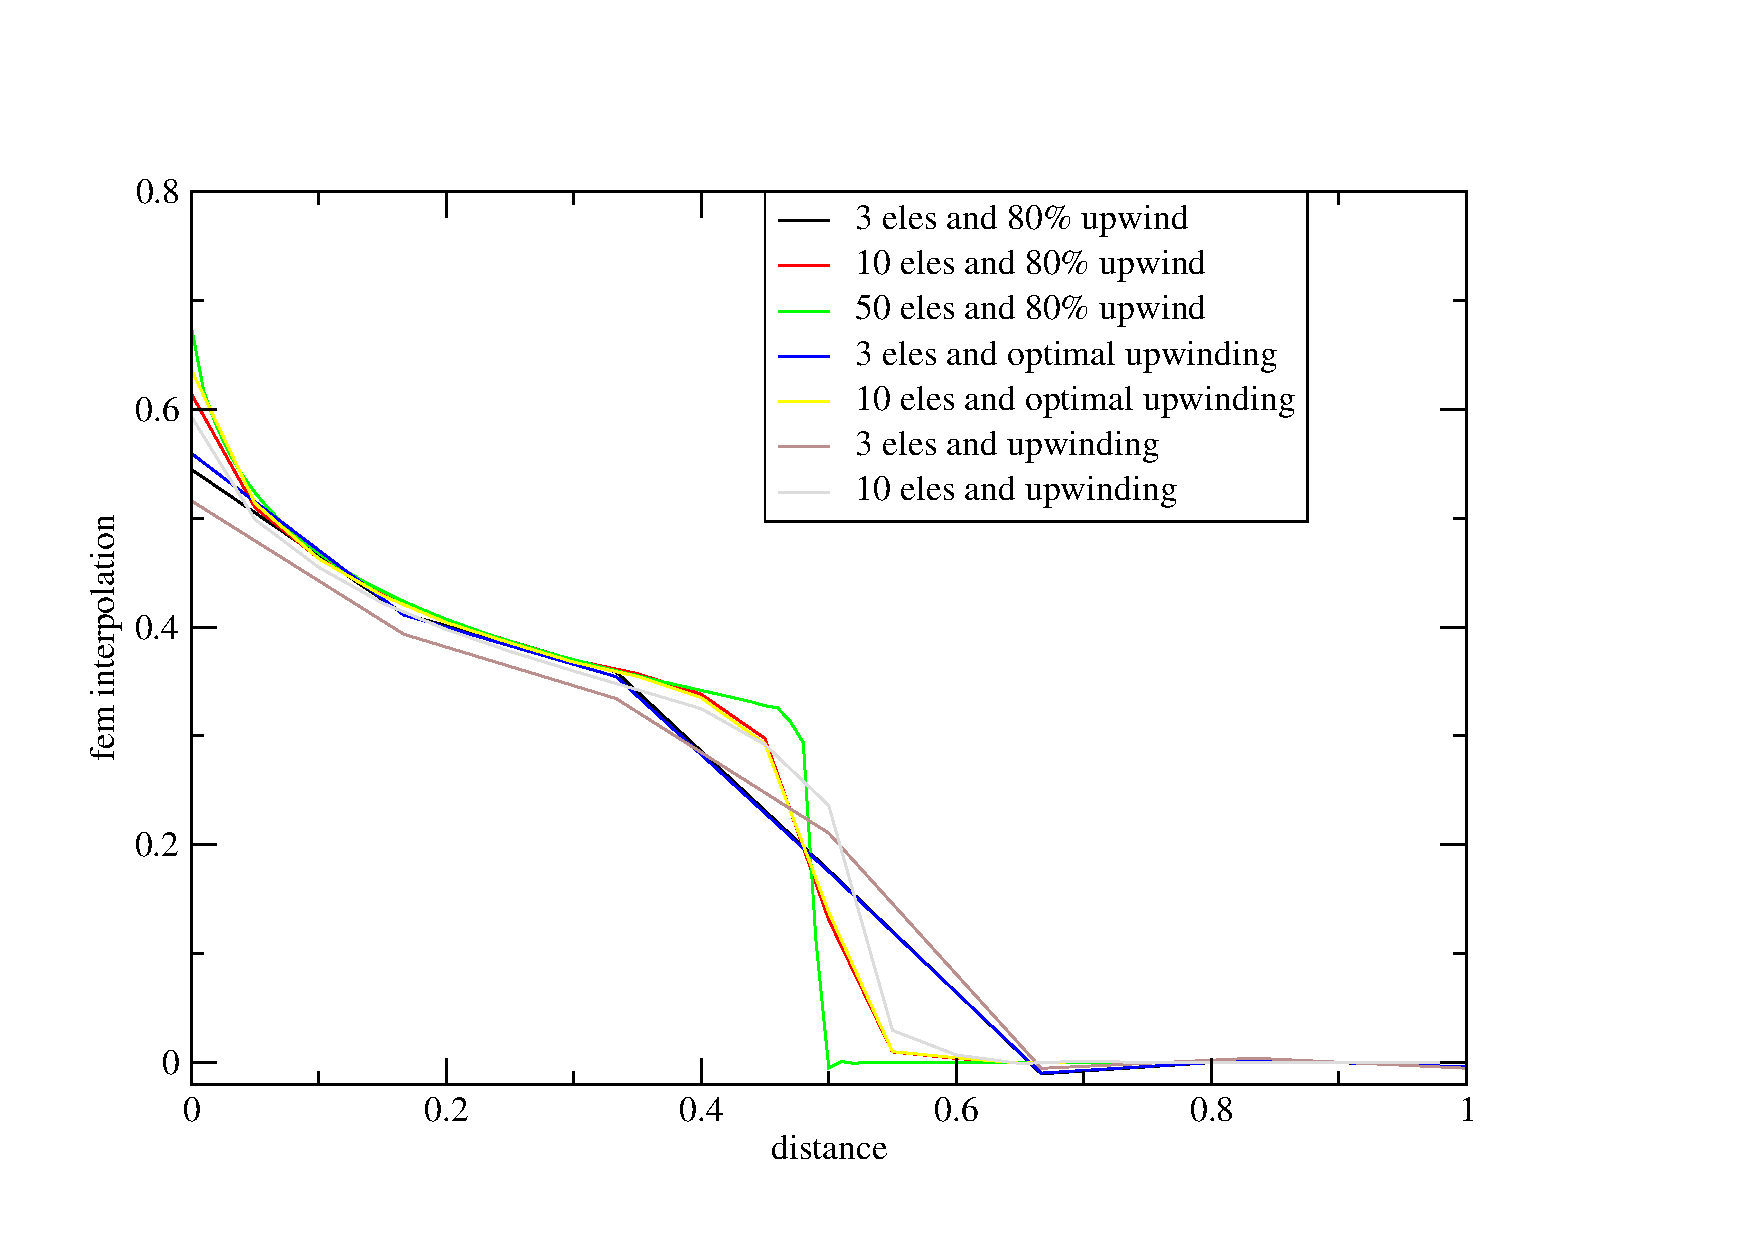
\includegraphics[width=17.5cm,height=12.5cm]{./doc_figures/bl-optimal-upwind}
\end{center}
\vspace{0.cm}}
\caption{Comparison of upwind, 80$\%$ upwind and optimal upwind solutions 
at various resolutions.  }
\label{bl-optimal-upwind}
\end{figure}

\begin{figure}[H]
\vbox{
\begin{center}
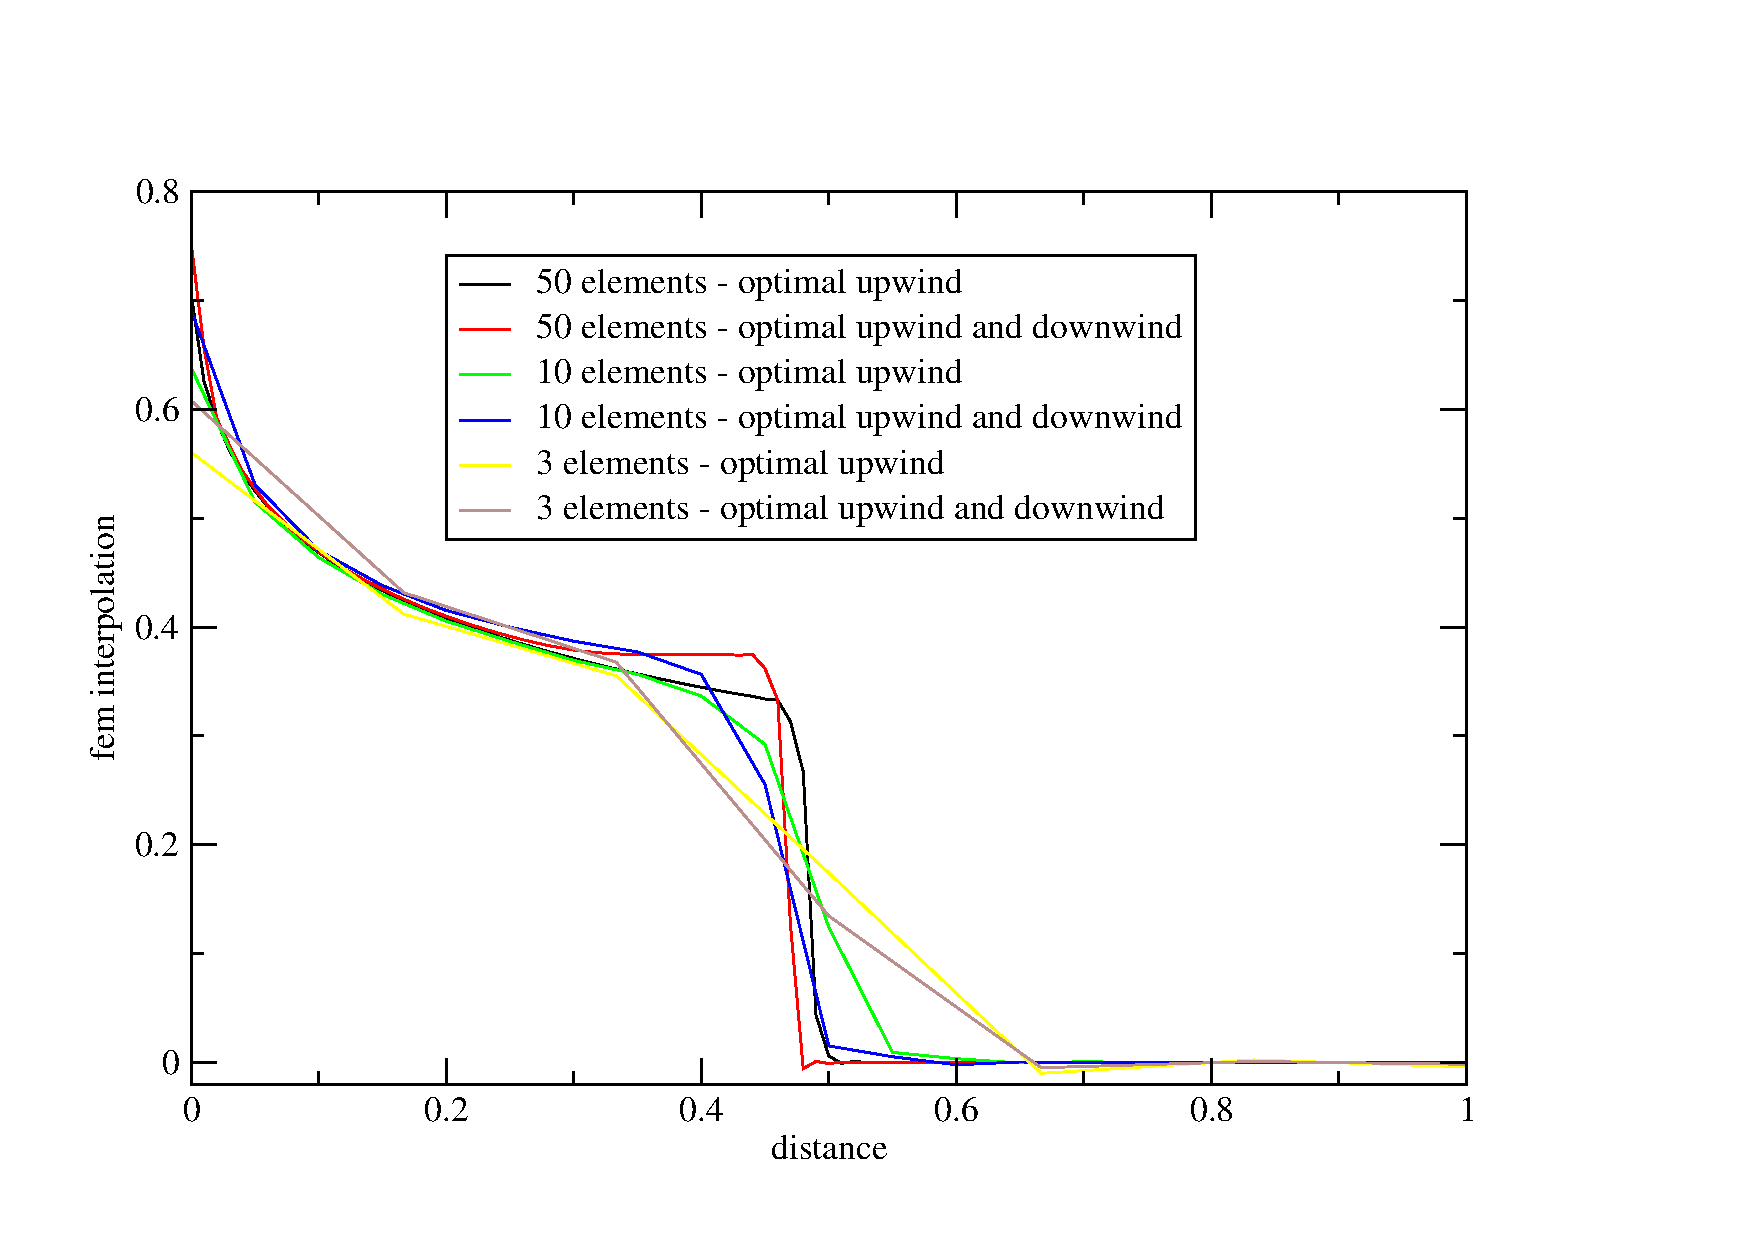
\includegraphics[width=17.5cm,height=12.5cm]{./doc_figures/bl-upwind-v-up-and-down}
\end{center}
\vspace{0.cm}}
\caption{A comparison of the optimal upwind formulation when using 
downwind as well as upwinding and upwinding only. The finite element interpolation 
of the gas saturation is shown at different mesh resolutions. 
Downwinding seems to detract from the accuracy of the solution. }
\label{bl-upwind-v-up-and-down}
\end{figure}

\begin{figure}[H]
\vbox{
\begin{center}
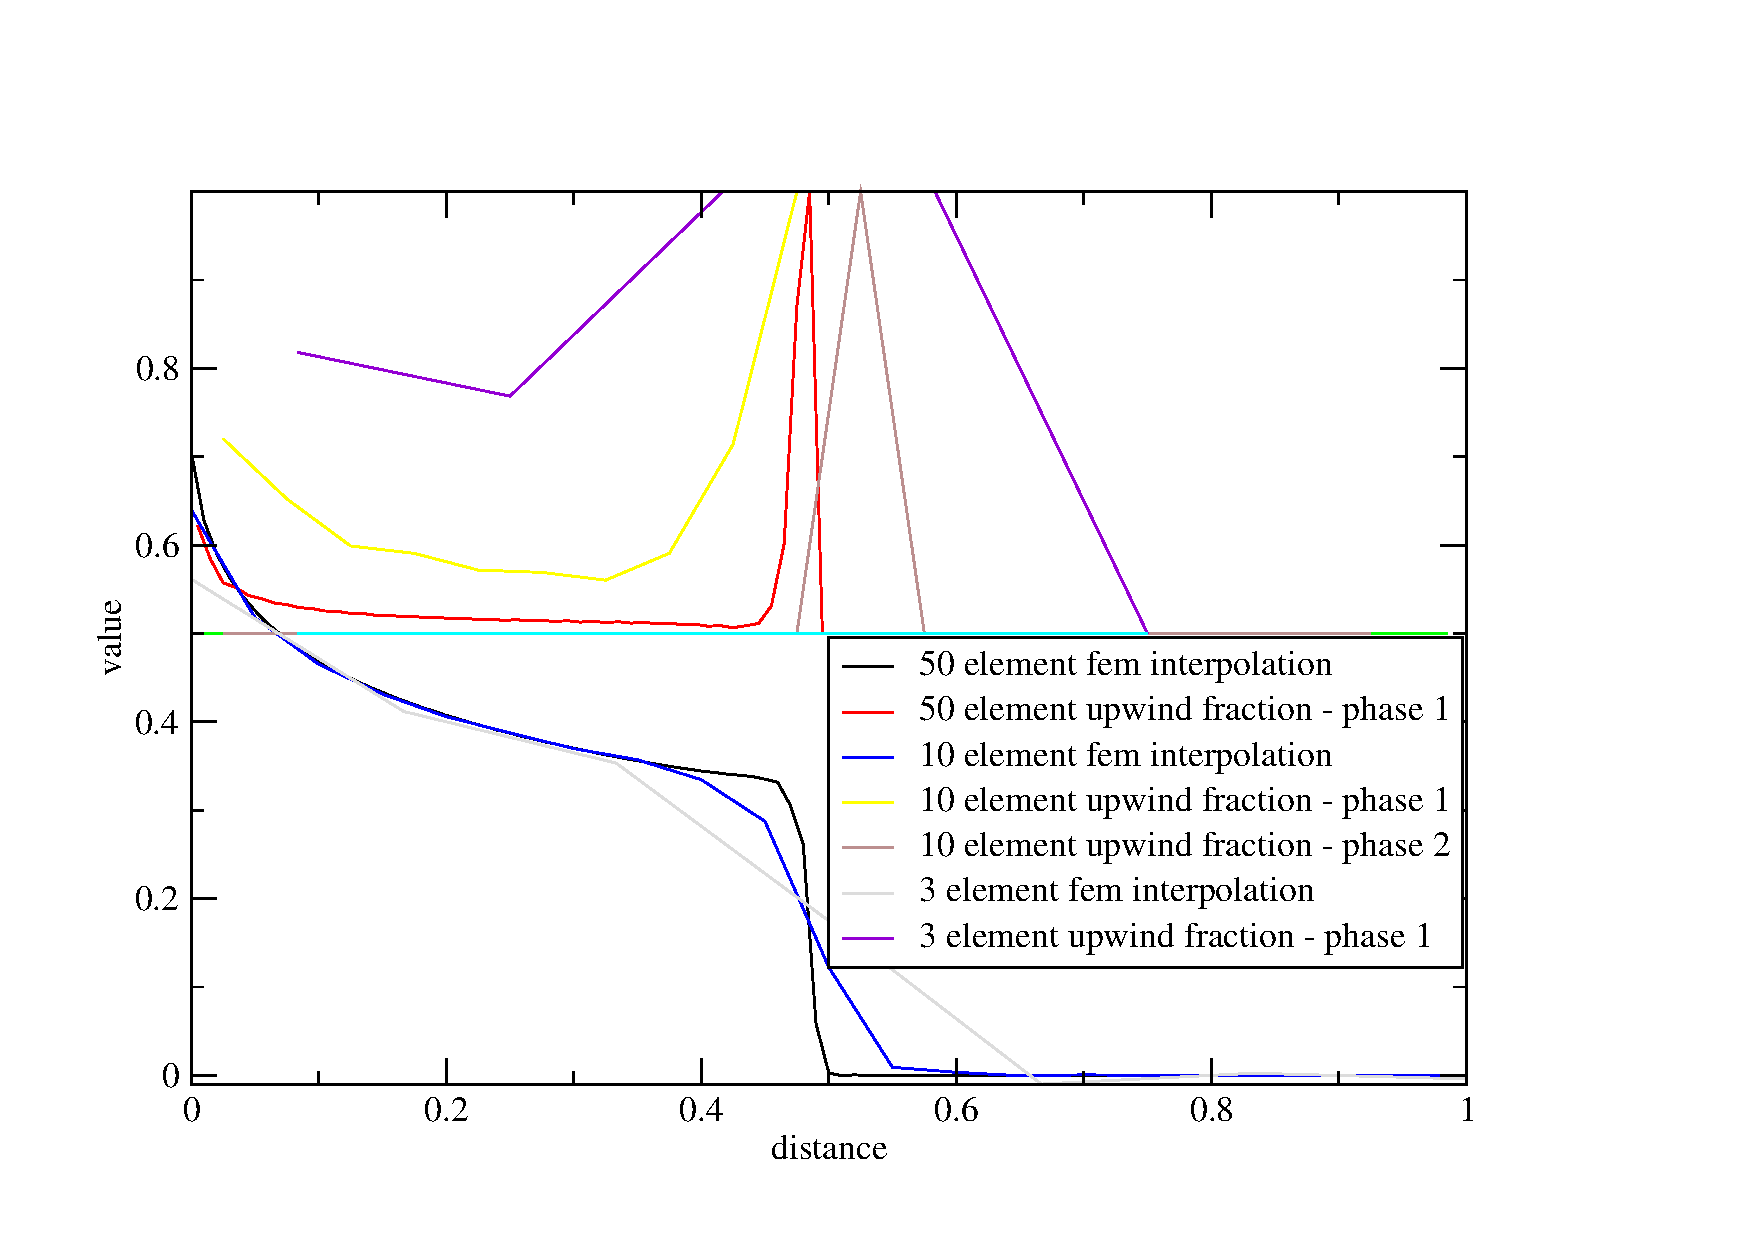
\includegraphics[width=17.5cm,height=12.5cm]{./doc_figures/bl-upwind-frac}
\end{center}
\vspace{0.cm}}
\caption{The fraction of upwinding used in the optimal upwinding approach at the control volume boundaries at the final time step and for three different mesh resolutions. Notice that the upwind fraction is at its largest near the shocks and is relatively small 
where the solution is smooth. The magnitude of the upwind fraction also reduces 
with increased mesh resolution. Also shown is the finite element interpolation 
of the gas saturation at the 3 mesh resolutions.  }
\label{bl-upwind-frac}
\end{figure}


\begin{figure}[H]
\vbox{
\begin{center}
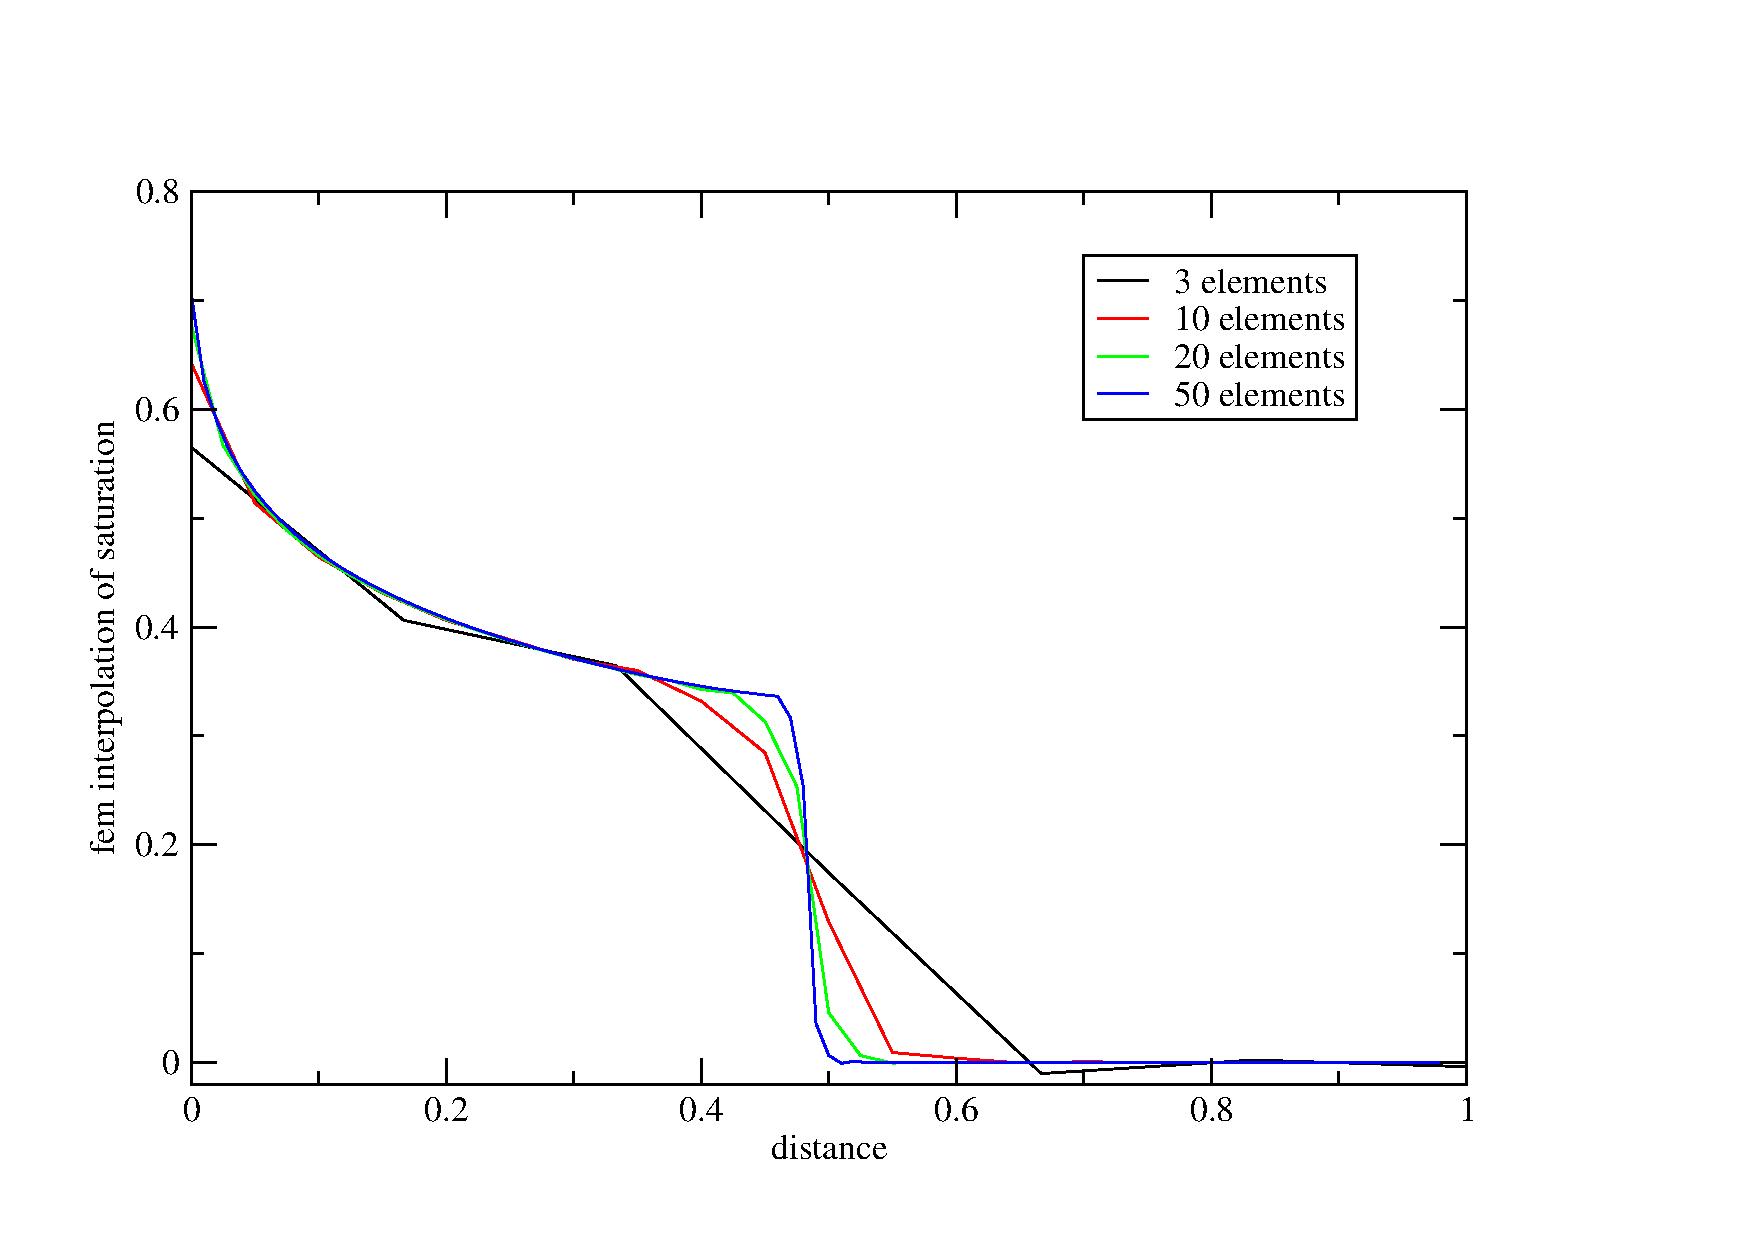
\includegraphics[width=17.5cm,height=12.5cm]{./doc_figures/bl-3-10-20-50}
\end{center}
\vspace{0.cm}}
\caption{The finite element interpolation of the gas volume fraction, for the optimal upwind scheme and for different mesh resolutions. }
\label{bl-3-10-20-50}
\end{figure}




\subsubsection{Discontinuous formulation}

Here results for the discontinuous between elements 
of saturation and pressure are presented. 
Having the discontinuity between elements potentially allows one 
to use a course mesh to represent abruptly changing fields. 
For example, using two discontinuous elements only one 
obtains a result, for the BL test case, which is qualatively 
similar to the converged solution, see \ref{bl-dg-2eles}. 
This solution was obtained with upwinding within and 
between the elements, as described in section \ref{opt-up}. 
This upwind scheme issued in all results presented here 
with the acception of solutions obtained using a central scheme 
as shown in figure \ref{bl-dg-cent-4-10-20} for different 
resolutions. The corresponding upwind solutions at the 
same mesh resolutions are shown in figure \ref{bl-dg-4-10-20}. 
In order to get a feel for how the discontinuous solutions 
compare, in terms of accuracy, with the continuous 
solutions of the previous subsection they are compared 
in figure \ref{bl-dg-4-10-vers-cty}. At the courser resolution 
they do seem more accurate despite the outstanding accuracy 
of the continuous formulation. We also show 
the accuracy of the formulation for linear fem-saturation/pressure and various mesh resolutions in figure \ref{bl-dg-p1-2-4-5-10-20-40}. 
Near the shock front there is little benefit in using high order elements 
so linear elements perform well here compared to quadratic elements. 

% dg:

%fig7: bl-dg-2eles.xmgr

%fig8: bl-dg-cent-4-10-20.xmgr

%fig9: bl-dg-4-10-20.xmgr

%fig10: bl-dg-4-10-vers-cty.xmgr



\begin{figure}[H]
\vbox{
\begin{center}
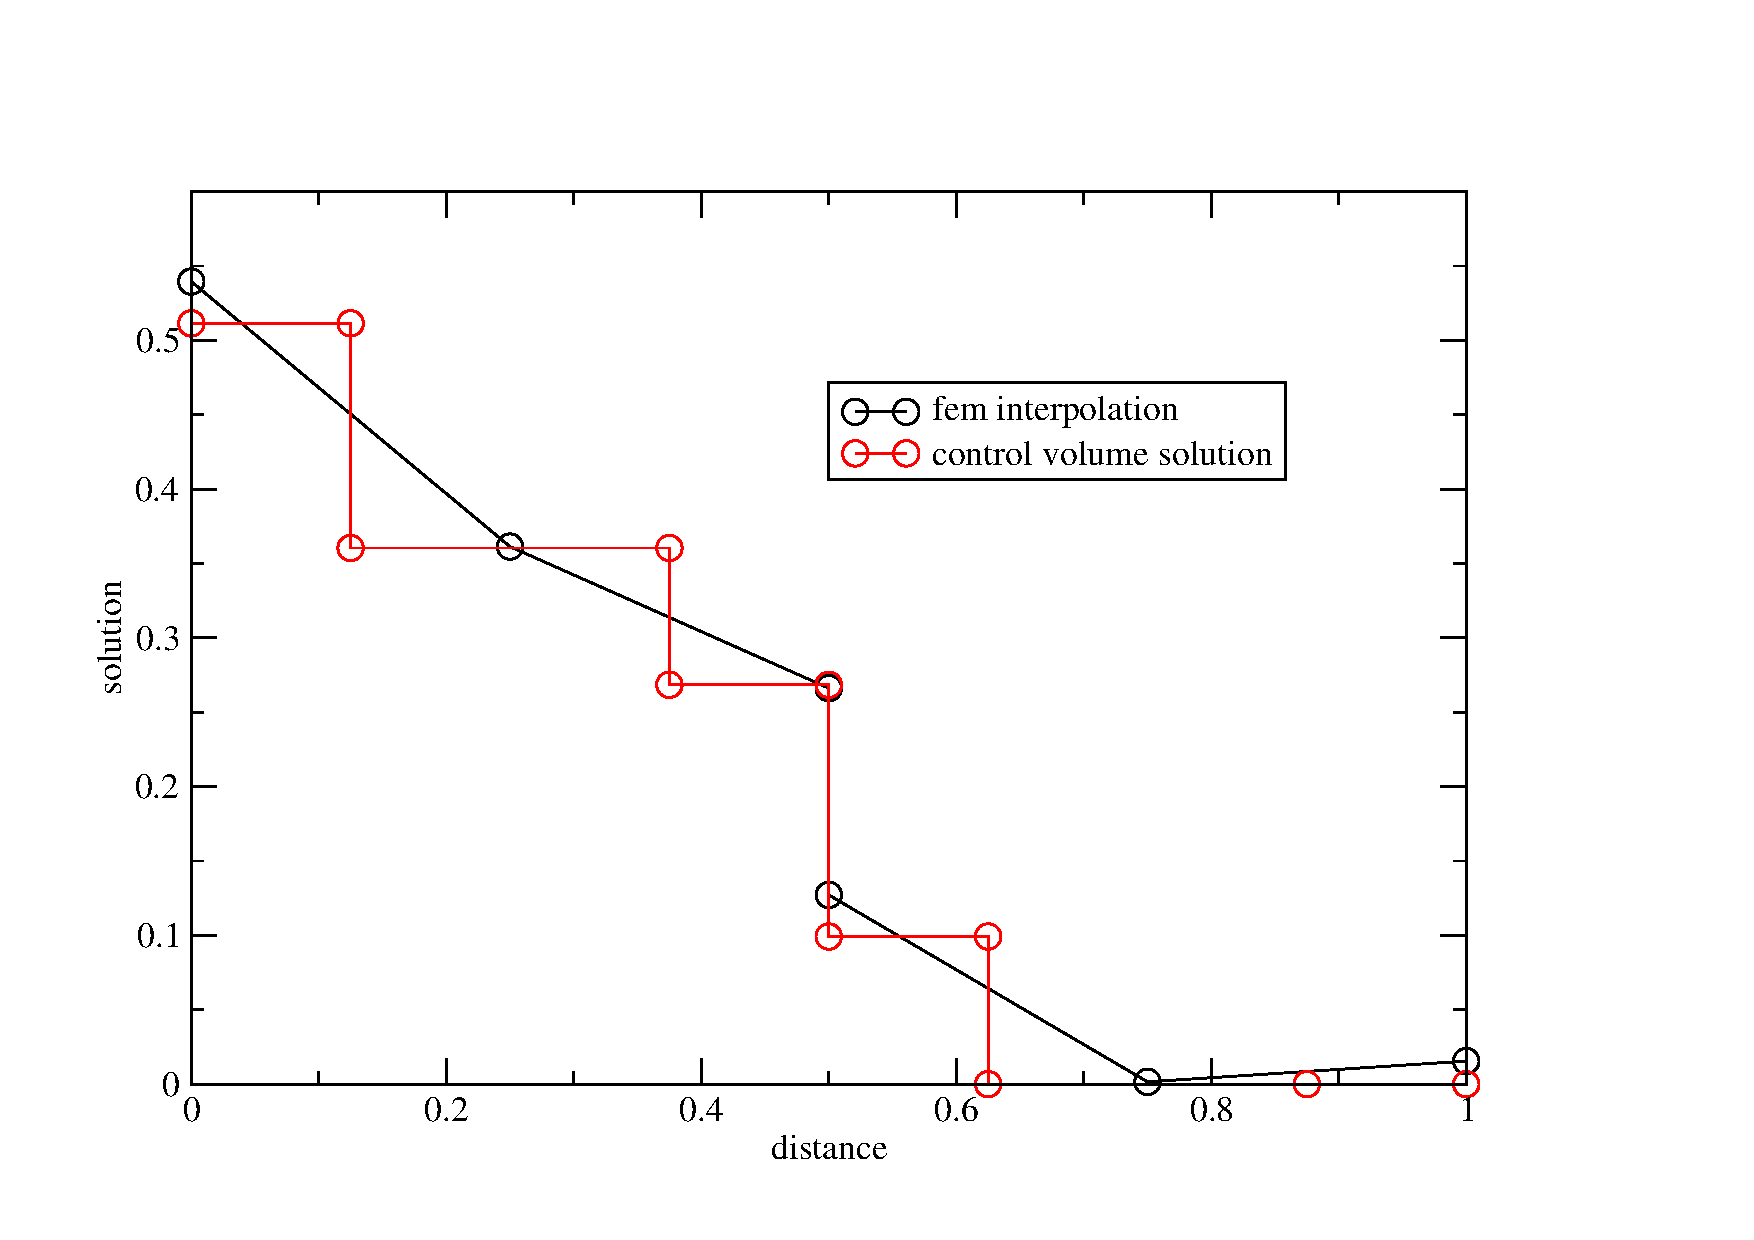
\includegraphics[width=17.5cm,height=12.5cm]{./doc_figures/bl-dg-2eles}
\end{center}
\vspace{0.cm}}
\caption{Two element solution using the discontinuous formulation. Both the 
control volume gas saturation and the finite element interpolation 
of this saturation are shown.  }
\label{bl-dg-2eles}
\end{figure}

\begin{figure}[H]
\vbox{
\begin{center}
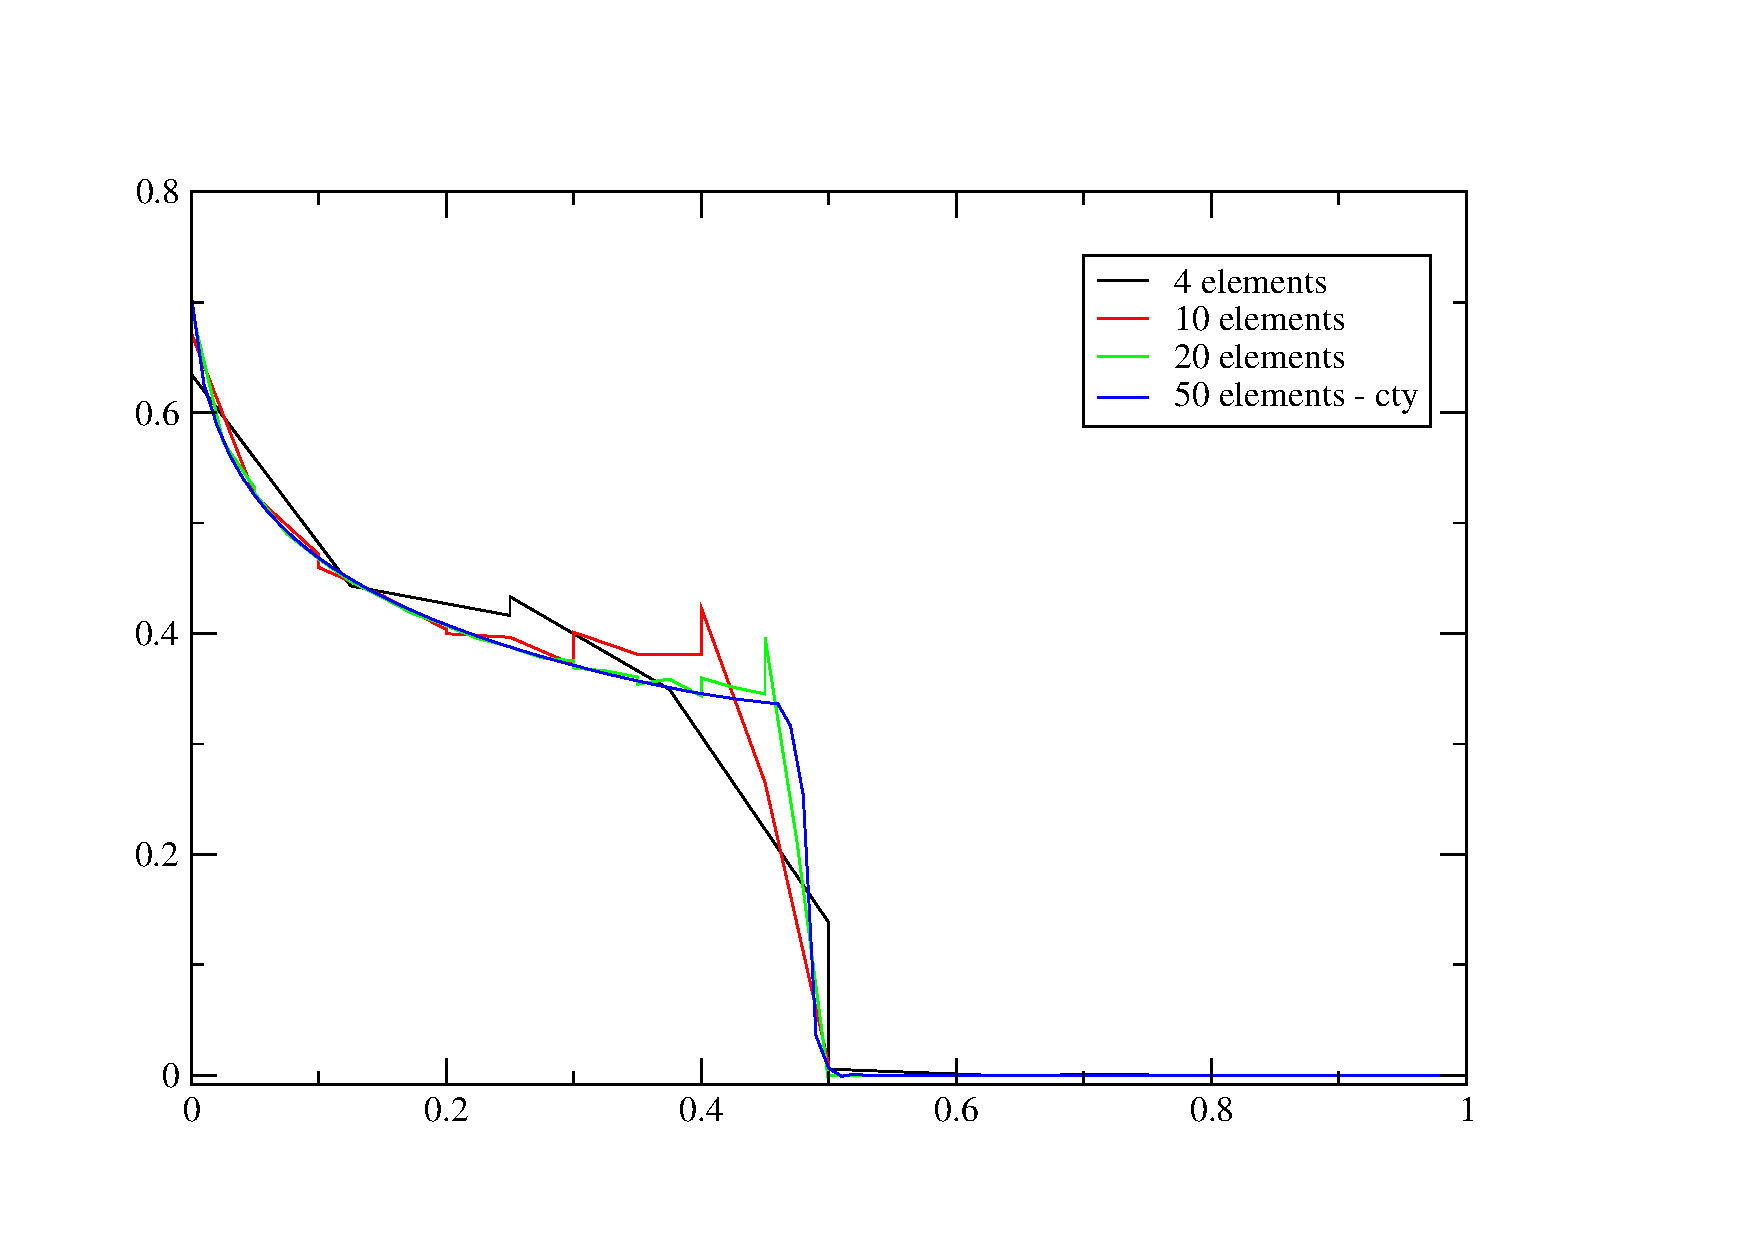
\includegraphics[width=17.5cm,height=12.5cm]{./doc_figures/bl-dg-cent-4-10-20}
\end{center}
\vspace{0.cm}}
\caption{Gas saturations from the discontinuous formulation with no upwinding and for 
different mesh resolutions. Notice that there are substantial oscillations.  }
\label{bl-dg-cent-4-10-20}
\end{figure}


\begin{figure}[H]
\vbox{
\begin{center}
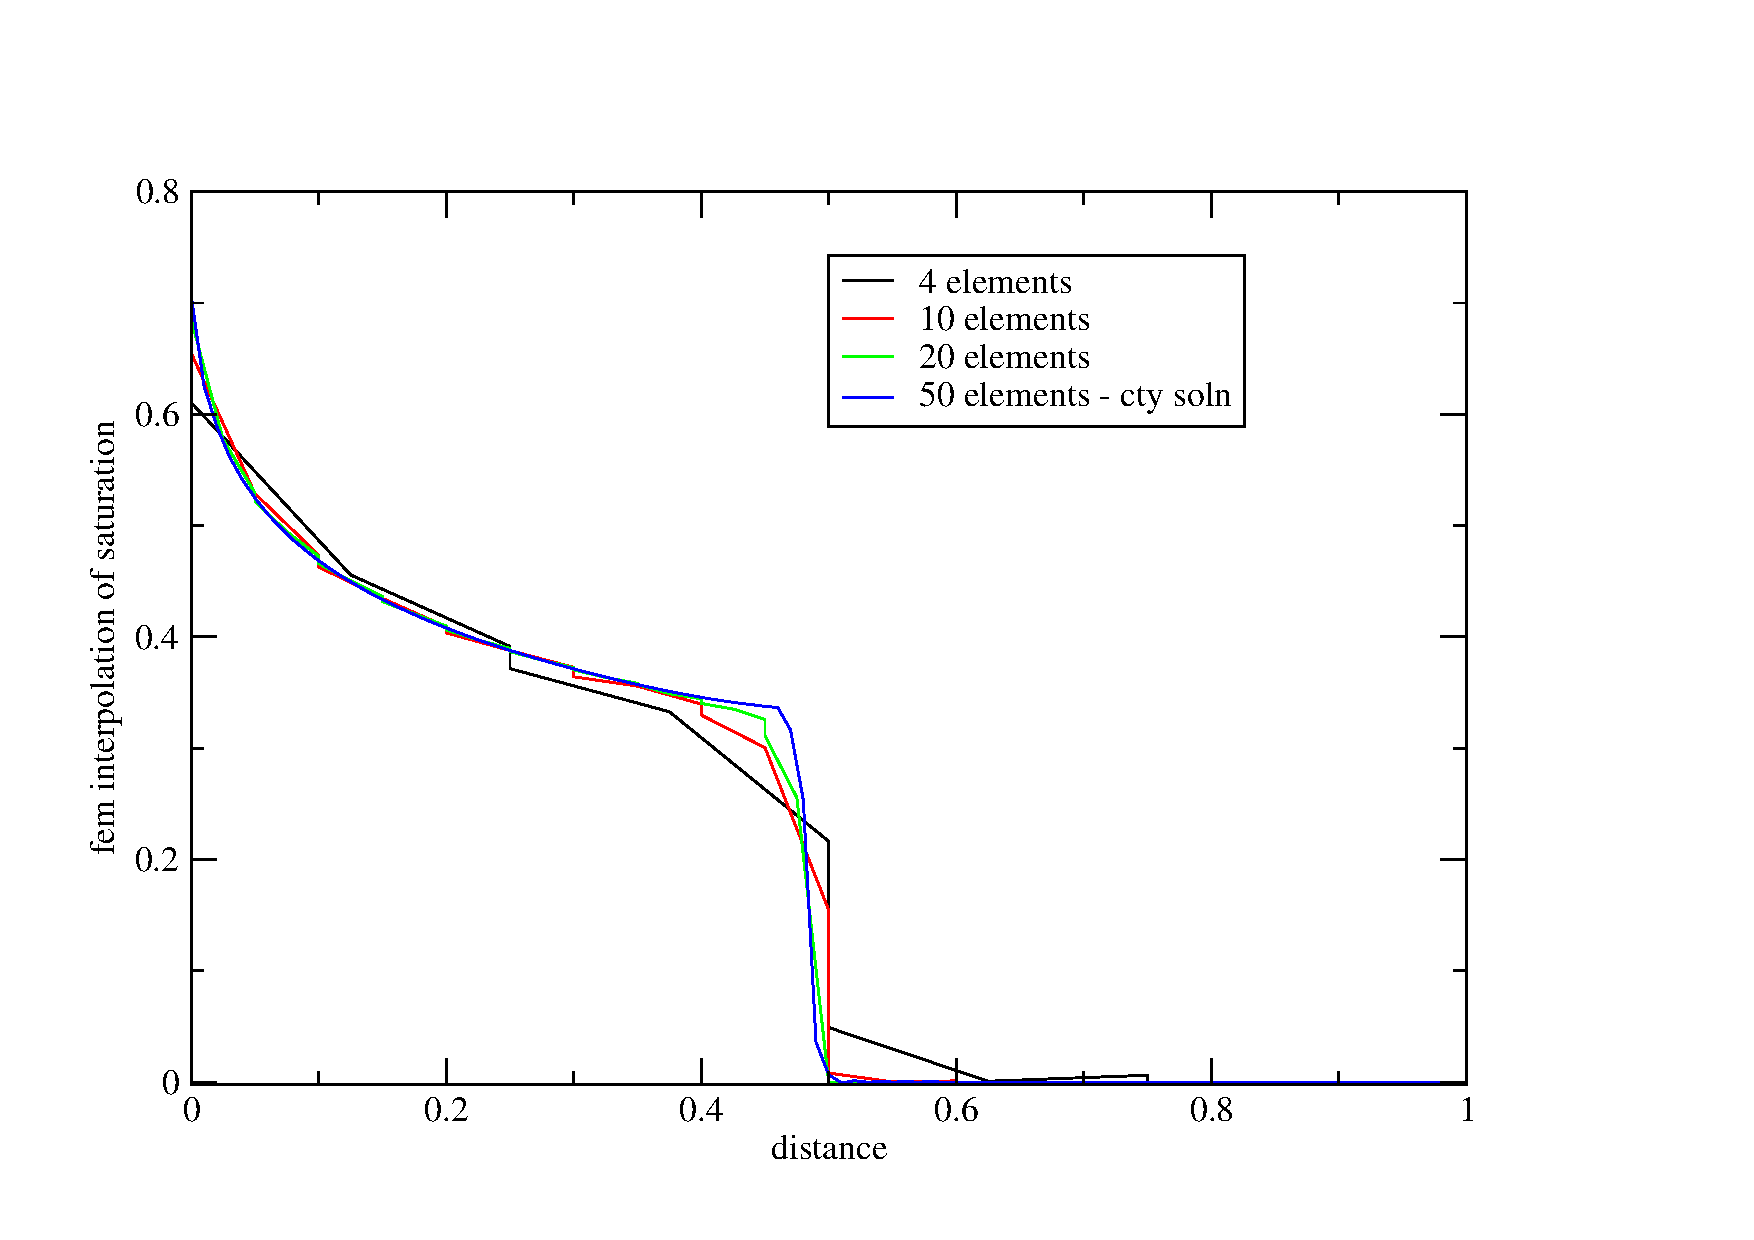
\includegraphics[width=17.5cm,height=12.5cm]{./doc_figures/bl-dg-4-10-20}
\end{center}
\vspace{0.cm}}
\caption{Gas saturations from the discontinuous formulation with upwinding and for 
different mesh resolutions.  
Notice that oscillations are suppressed compared to the central scheme.  }
\label{bl-dg-4-10-20}
\end{figure}


\begin{figure}[H]
\vbox{
\begin{center}
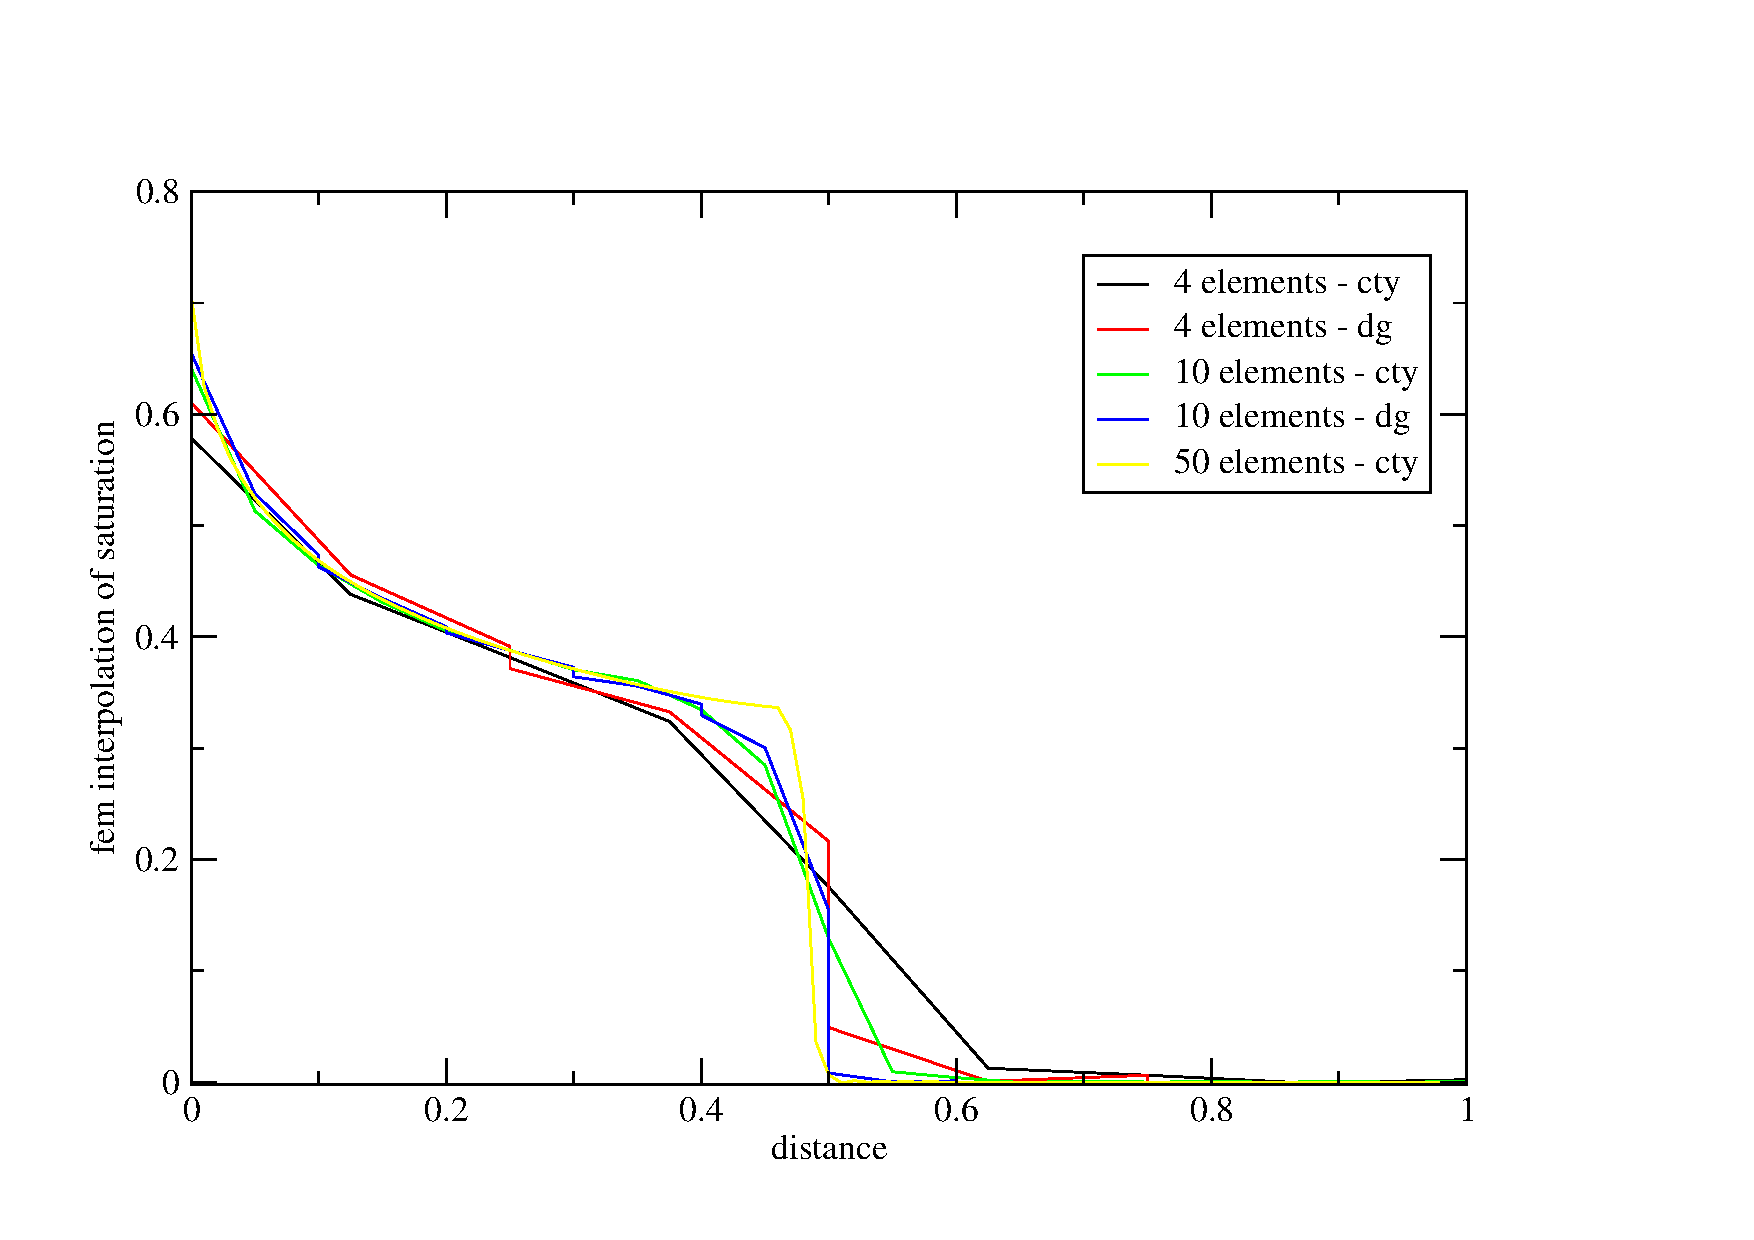
\includegraphics[width=17.5cm,height=12.5cm]{./doc_figures/bl-dg-4-10-vers-cty}
\end{center}
\vspace{0.cm}}
\caption{Gas saturations shown comparing the accuracy of the discontinuous between elements and continuous 
formulation. The 50 element continuous solution may be viewed as a converged 
result.     }
\label{bl-dg-4-10-vers-cty}
\end{figure}


\begin{figure}[H]
\vbox{
\begin{center}
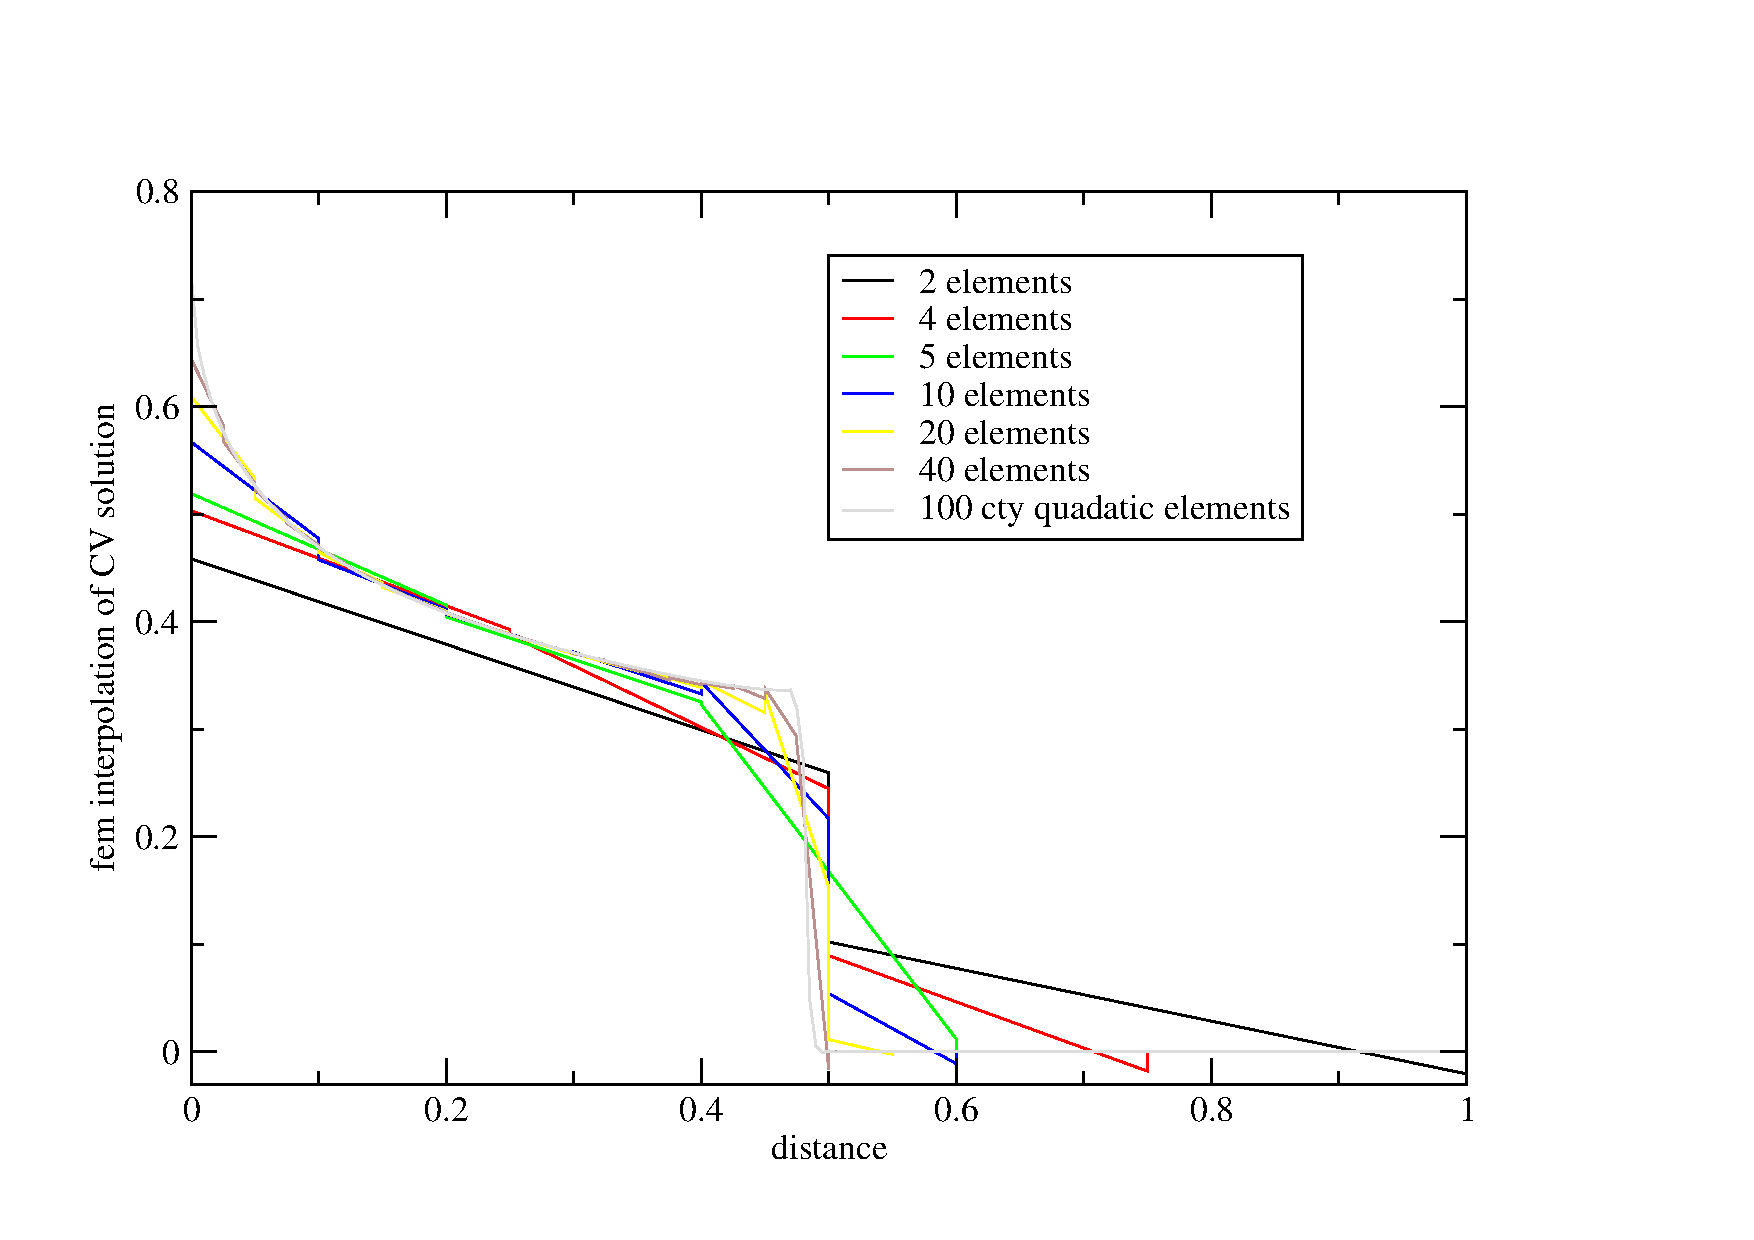
\includegraphics[width=17.5cm,height=12.5cm]{./doc_figures/bl-dg-p1-2-4-5-10-20-40}
\end{center}
\vspace{0.cm}}
\caption{Gas saturations for p1(linear) pressure/(fem-interpolation of saturation) 
for changing mesh resolution.   }
\label{bl-dg-p1-2-4-5-10-20-40}
\end{figure}


%\pagebreak


\subsubsection{BL test case with positive and negative gravity} 

In this section we apply the the formulations to the test 
case of the previous section but with gravity defined 
in both the negative (figure \ref{bl-sou-neg}) and 
positive (figure \ref{bl-sou-pos}) x-directions. 
These solutions converge to the analytical solutions 
shown in the appendix. 
Notice that for the negative gravity source the less dense gas region 
is compressed (compared to the case without gravity shown in 
the previous section) by the weight of the more dense liquid and 
the opposite happens for the positive gravity result. 


\begin{figure}[H]
\vbox{
\begin{center}
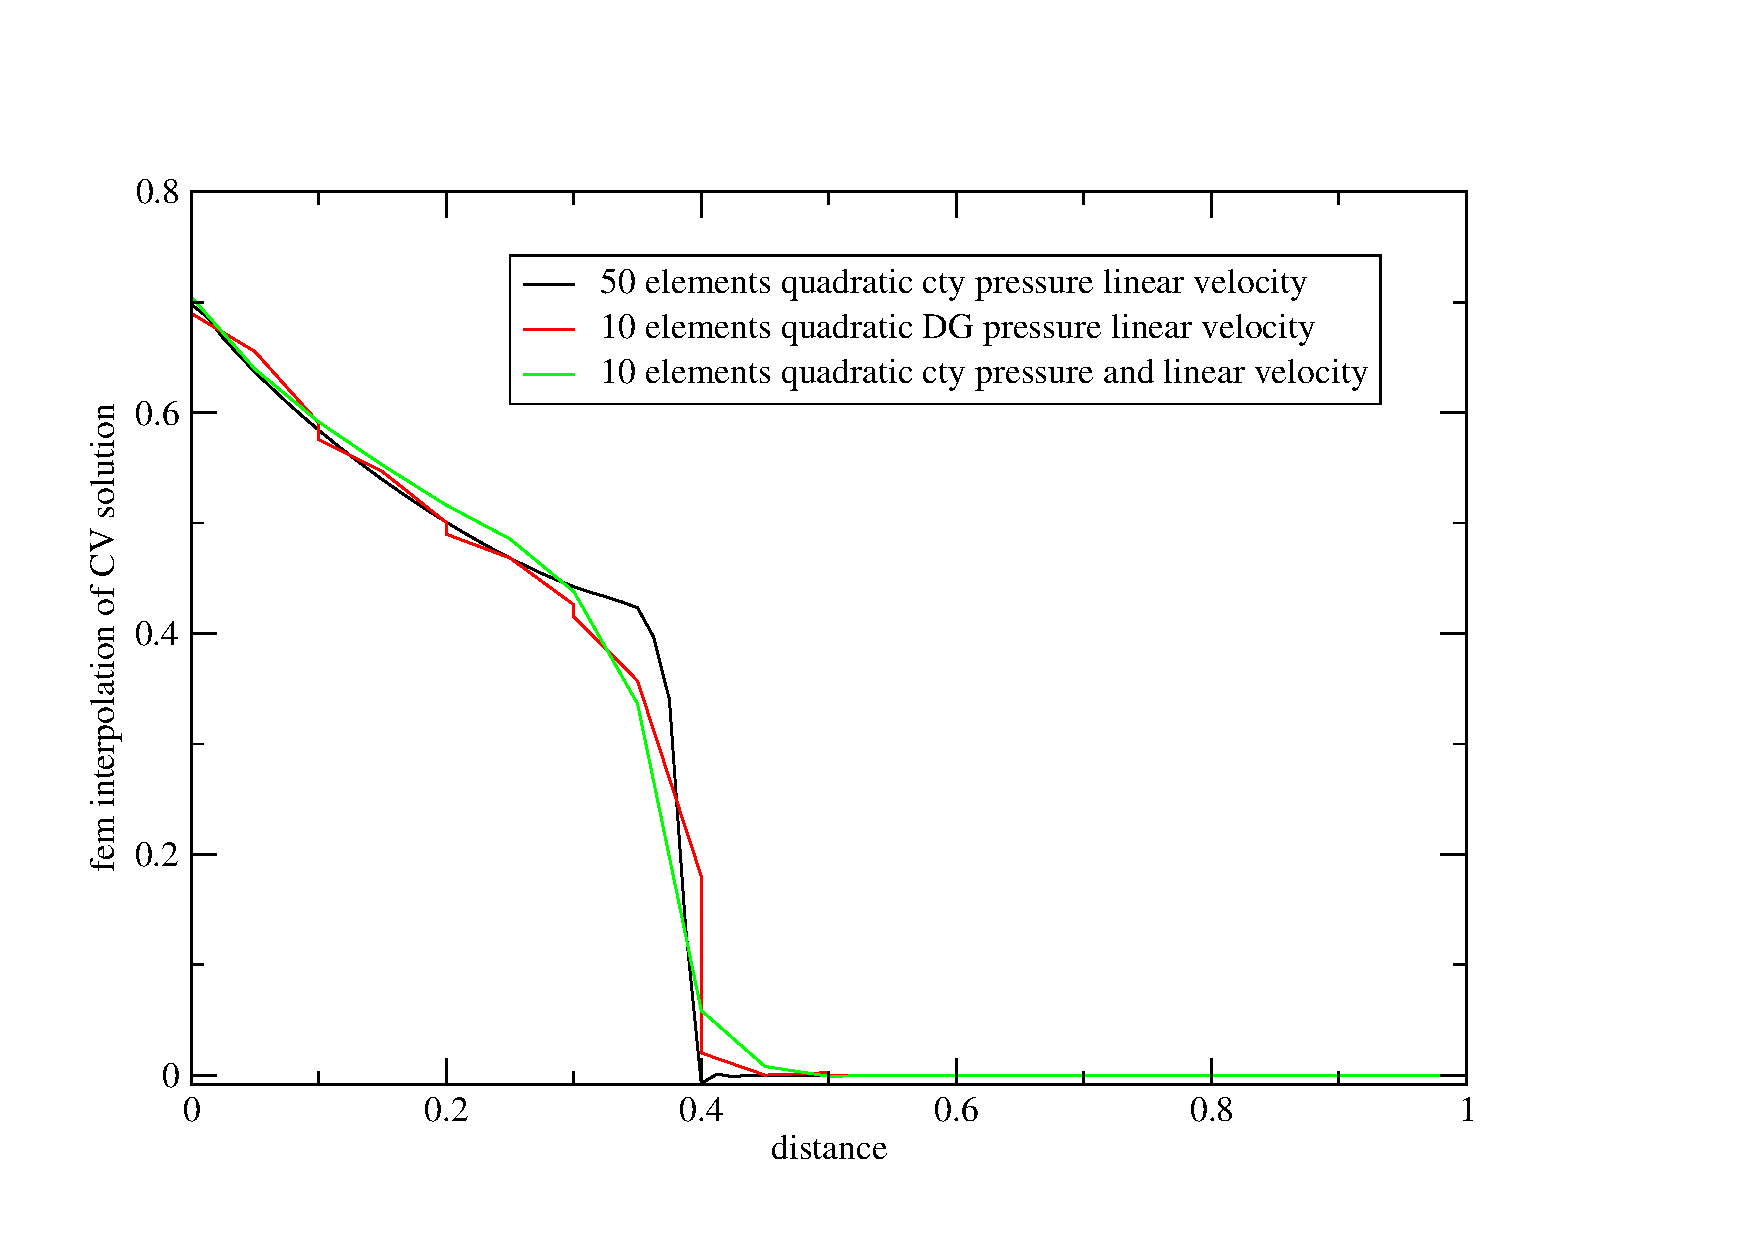
\includegraphics[width=17.5cm,height=12.5cm]{./doc_figures/bl-sou-pos}
\end{center}
\vspace{0.cm}}
\caption{Gas saturations for p2(quadratic) pressure/(fem-interpolation of saturation) 
for changing mesh resolution and for the test case with gravity acting in 
the +ve x-direction. }
\label{bl-sou-pos}
\end{figure}


\begin{figure}[H]
\vbox{
\begin{center}
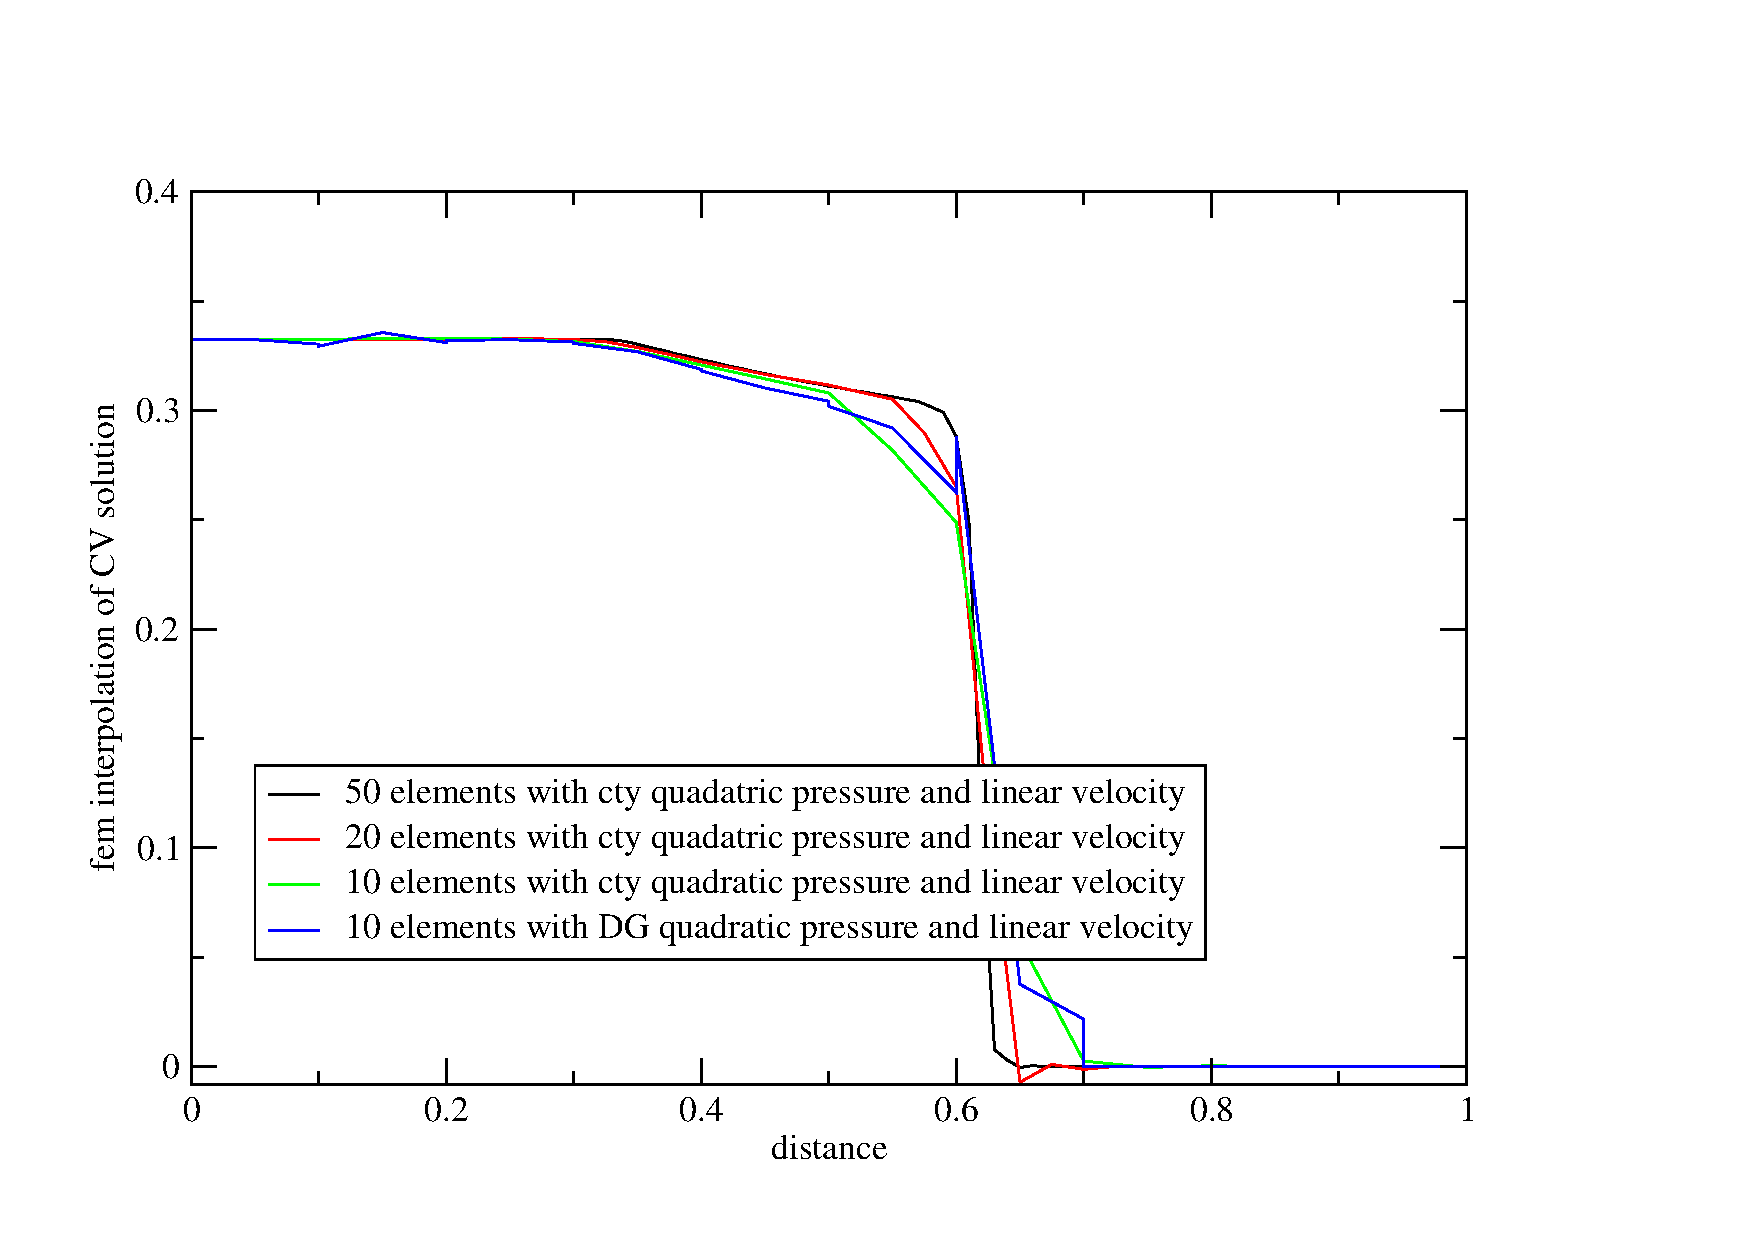
\includegraphics[width=17.5cm,height=12.5cm]{./doc_figures/bl-sou-neg}
\end{center}
\vspace{0.cm}}
\caption{Gas saturations for p2(quadratic) pressure/(fem-interpolation of saturation) 
for changing mesh resolution and for the test case with gravity acting in 
the -ve x-direction. }
\label{bl-sou-neg}
\end{figure}


\subsubsection{Pressure/density wave propogation} 

In this section we solve a single phase flow problem 
with an compressible with a simple EoS given by 
$\rho=1+0.01 p_{CV}$ and the fluid initially as rest. 
The inlet velocity is accelerated within 
one time step (the time step sizes are $\Delta t=1\times 10^{-4}$) 
to a unit velocity and is sustained for 0.005 seconds. 
The inlet velocity is then decreased to zero. 
The rest is a density/pressure wave which 
propagates across the domain with a characteristic 
velocity of $c=10$. The results at $t=0.25$ seconds 
into the simulation are shown. The outlet pressure is zero 
and initial density unity. 

An intermediate density using a quadratic DG pressure 
and cubic DG velocity are shown in figure \ref{compres-imp-nonlin}. 
The final solution is shown for this scheme as well 
as a quadratic continuous pressure and quadratic DG velocity 
scheme. In addition, we use the same two scheme's but 
switching off the non-linear terms in the momentum 
equations (retaining the time term only) to 
produce the results shown in figure \ref{compres-imp-no-nonlin}. We have 
also shown the results using the overlapping finite 
element method. For the continuous scheme this results 
in an exact representation of the momentum equation.  
For the DG pressure formulation this is no longer 
true but is close in some sense. 


\begin{figure}[H]
\vbox{
\begin{center}
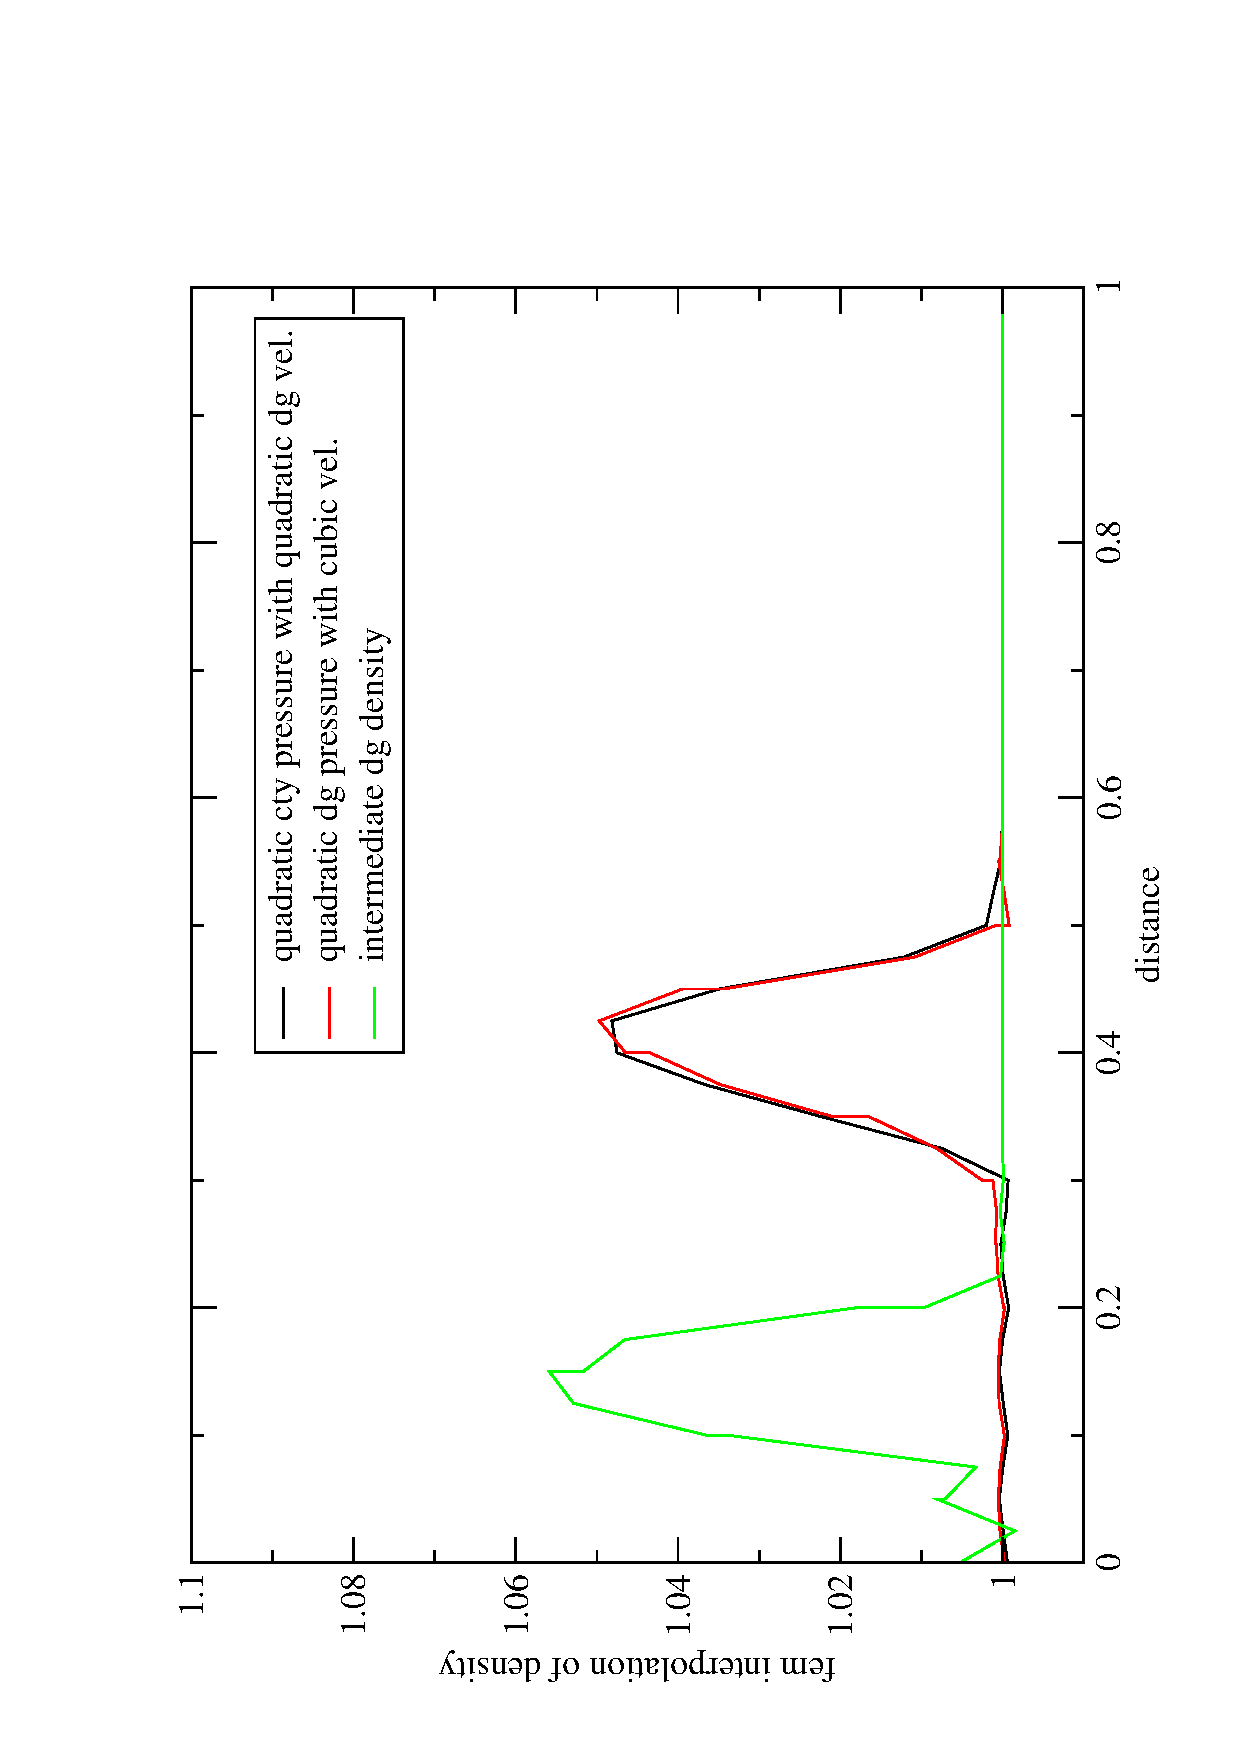
\includegraphics[width=17.5cm,height=12.5cm]{./doc_figures/compres-imp-nonlin}
\end{center}
\vspace{0.cm}}
\caption{Density wave propogation from left to right across the domain 
with DG and continuous pressure formulations. The fem-interpolation of 
density is shown. }
\label{compres-imp-nonlin}
\end{figure}


\begin{figure}[H]
\vbox{
\begin{center}
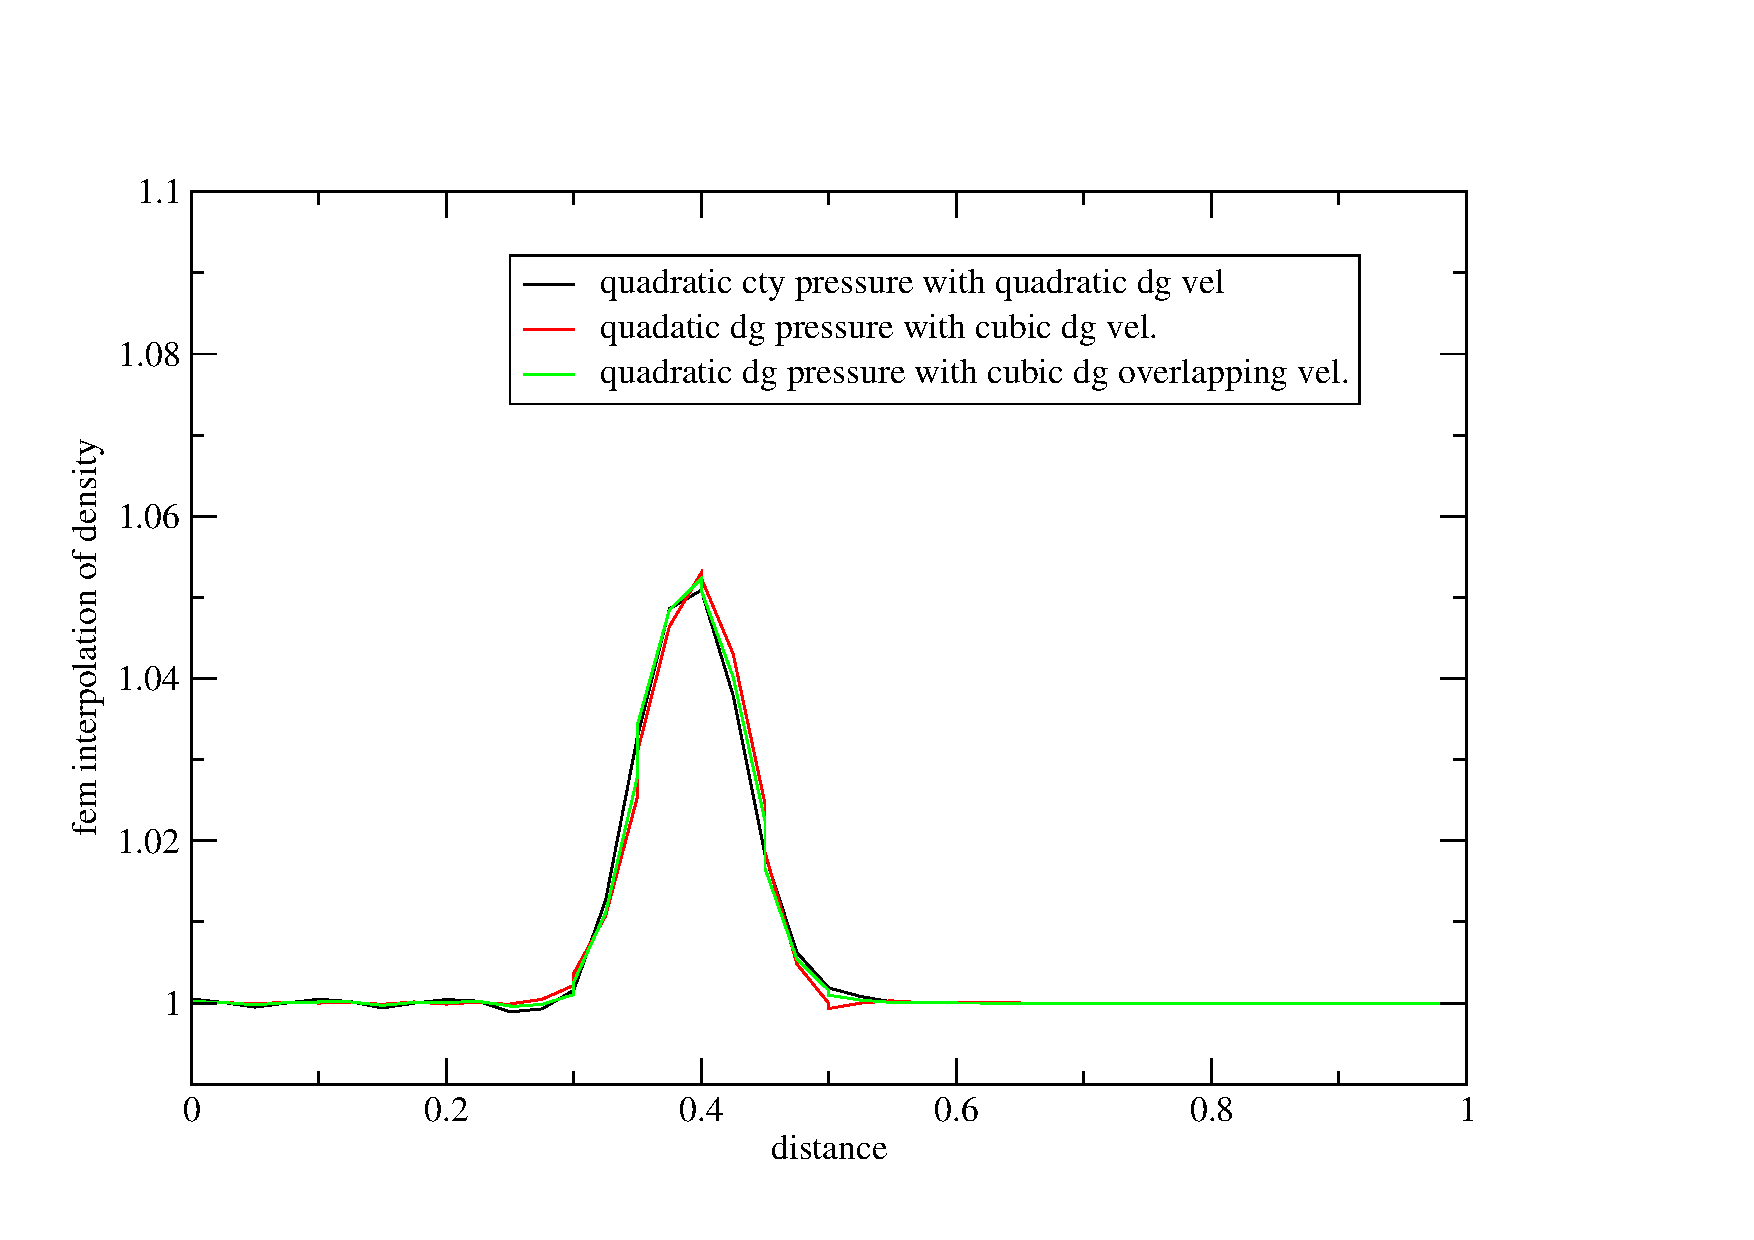
\includegraphics[width=17.5cm,height=12.5cm]{./doc_figures/compres-imp-no-nonlin}
\end{center}
\vspace{0.cm}}
\caption{Density wave propogation from left to right across the domain 
with DG, continuous pressure and overlapping velocity formulations. 
The non-linear terms in the momentum equations are switched off 
in these simulations. The fem-interpolation of 
density is shown.  }
\label{compres-imp-no-nonlin}
\end{figure}

